% Options for packages loaded elsewhere
\PassOptionsToPackage{unicode}{hyperref}
\PassOptionsToPackage{hyphens}{url}
\PassOptionsToPackage{dvipsnames,svgnames,x11names}{xcolor}
%
\documentclass[
  letterpaper,
  DIV=11,
  numbers=noendperiod]{scrartcl}

\usepackage{amsmath,amssymb}
\usepackage{iftex}
\ifPDFTeX
  \usepackage[T1]{fontenc}
  \usepackage[utf8]{inputenc}
  \usepackage{textcomp} % provide euro and other symbols
\else % if luatex or xetex
  \usepackage{unicode-math}
  \defaultfontfeatures{Scale=MatchLowercase}
  \defaultfontfeatures[\rmfamily]{Ligatures=TeX,Scale=1}
\fi
\usepackage{lmodern}
\ifPDFTeX\else  
    % xetex/luatex font selection
\fi
% Use upquote if available, for straight quotes in verbatim environments
\IfFileExists{upquote.sty}{\usepackage{upquote}}{}
\IfFileExists{microtype.sty}{% use microtype if available
  \usepackage[]{microtype}
  \UseMicrotypeSet[protrusion]{basicmath} % disable protrusion for tt fonts
}{}
\makeatletter
\@ifundefined{KOMAClassName}{% if non-KOMA class
  \IfFileExists{parskip.sty}{%
    \usepackage{parskip}
  }{% else
    \setlength{\parindent}{0pt}
    \setlength{\parskip}{6pt plus 2pt minus 1pt}}
}{% if KOMA class
  \KOMAoptions{parskip=half}}
\makeatother
\usepackage{xcolor}
\setlength{\emergencystretch}{3em} % prevent overfull lines
\setcounter{secnumdepth}{-\maxdimen} % remove section numbering
% Make \paragraph and \subparagraph free-standing
\ifx\paragraph\undefined\else
  \let\oldparagraph\paragraph
  \renewcommand{\paragraph}[1]{\oldparagraph{#1}\mbox{}}
\fi
\ifx\subparagraph\undefined\else
  \let\oldsubparagraph\subparagraph
  \renewcommand{\subparagraph}[1]{\oldsubparagraph{#1}\mbox{}}
\fi

\usepackage{color}
\usepackage{fancyvrb}
\newcommand{\VerbBar}{|}
\newcommand{\VERB}{\Verb[commandchars=\\\{\}]}
\DefineVerbatimEnvironment{Highlighting}{Verbatim}{commandchars=\\\{\}}
% Add ',fontsize=\small' for more characters per line
\usepackage{framed}
\definecolor{shadecolor}{RGB}{241,243,245}
\newenvironment{Shaded}{\begin{snugshade}}{\end{snugshade}}
\newcommand{\AlertTok}[1]{\textcolor[rgb]{0.68,0.00,0.00}{#1}}
\newcommand{\AnnotationTok}[1]{\textcolor[rgb]{0.37,0.37,0.37}{#1}}
\newcommand{\AttributeTok}[1]{\textcolor[rgb]{0.40,0.45,0.13}{#1}}
\newcommand{\BaseNTok}[1]{\textcolor[rgb]{0.68,0.00,0.00}{#1}}
\newcommand{\BuiltInTok}[1]{\textcolor[rgb]{0.00,0.23,0.31}{#1}}
\newcommand{\CharTok}[1]{\textcolor[rgb]{0.13,0.47,0.30}{#1}}
\newcommand{\CommentTok}[1]{\textcolor[rgb]{0.37,0.37,0.37}{#1}}
\newcommand{\CommentVarTok}[1]{\textcolor[rgb]{0.37,0.37,0.37}{\textit{#1}}}
\newcommand{\ConstantTok}[1]{\textcolor[rgb]{0.56,0.35,0.01}{#1}}
\newcommand{\ControlFlowTok}[1]{\textcolor[rgb]{0.00,0.23,0.31}{#1}}
\newcommand{\DataTypeTok}[1]{\textcolor[rgb]{0.68,0.00,0.00}{#1}}
\newcommand{\DecValTok}[1]{\textcolor[rgb]{0.68,0.00,0.00}{#1}}
\newcommand{\DocumentationTok}[1]{\textcolor[rgb]{0.37,0.37,0.37}{\textit{#1}}}
\newcommand{\ErrorTok}[1]{\textcolor[rgb]{0.68,0.00,0.00}{#1}}
\newcommand{\ExtensionTok}[1]{\textcolor[rgb]{0.00,0.23,0.31}{#1}}
\newcommand{\FloatTok}[1]{\textcolor[rgb]{0.68,0.00,0.00}{#1}}
\newcommand{\FunctionTok}[1]{\textcolor[rgb]{0.28,0.35,0.67}{#1}}
\newcommand{\ImportTok}[1]{\textcolor[rgb]{0.00,0.46,0.62}{#1}}
\newcommand{\InformationTok}[1]{\textcolor[rgb]{0.37,0.37,0.37}{#1}}
\newcommand{\KeywordTok}[1]{\textcolor[rgb]{0.00,0.23,0.31}{#1}}
\newcommand{\NormalTok}[1]{\textcolor[rgb]{0.00,0.23,0.31}{#1}}
\newcommand{\OperatorTok}[1]{\textcolor[rgb]{0.37,0.37,0.37}{#1}}
\newcommand{\OtherTok}[1]{\textcolor[rgb]{0.00,0.23,0.31}{#1}}
\newcommand{\PreprocessorTok}[1]{\textcolor[rgb]{0.68,0.00,0.00}{#1}}
\newcommand{\RegionMarkerTok}[1]{\textcolor[rgb]{0.00,0.23,0.31}{#1}}
\newcommand{\SpecialCharTok}[1]{\textcolor[rgb]{0.37,0.37,0.37}{#1}}
\newcommand{\SpecialStringTok}[1]{\textcolor[rgb]{0.13,0.47,0.30}{#1}}
\newcommand{\StringTok}[1]{\textcolor[rgb]{0.13,0.47,0.30}{#1}}
\newcommand{\VariableTok}[1]{\textcolor[rgb]{0.07,0.07,0.07}{#1}}
\newcommand{\VerbatimStringTok}[1]{\textcolor[rgb]{0.13,0.47,0.30}{#1}}
\newcommand{\WarningTok}[1]{\textcolor[rgb]{0.37,0.37,0.37}{\textit{#1}}}

\providecommand{\tightlist}{%
  \setlength{\itemsep}{0pt}\setlength{\parskip}{0pt}}\usepackage{longtable,booktabs,array}
\usepackage{calc} % for calculating minipage widths
% Correct order of tables after \paragraph or \subparagraph
\usepackage{etoolbox}
\makeatletter
\patchcmd\longtable{\par}{\if@noskipsec\mbox{}\fi\par}{}{}
\makeatother
% Allow footnotes in longtable head/foot
\IfFileExists{footnotehyper.sty}{\usepackage{footnotehyper}}{\usepackage{footnote}}
\makesavenoteenv{longtable}
\usepackage{graphicx}
\makeatletter
\def\maxwidth{\ifdim\Gin@nat@width>\linewidth\linewidth\else\Gin@nat@width\fi}
\def\maxheight{\ifdim\Gin@nat@height>\textheight\textheight\else\Gin@nat@height\fi}
\makeatother
% Scale images if necessary, so that they will not overflow the page
% margins by default, and it is still possible to overwrite the defaults
% using explicit options in \includegraphics[width, height, ...]{}
\setkeys{Gin}{width=\maxwidth,height=\maxheight,keepaspectratio}
% Set default figure placement to htbp
\makeatletter
\def\fps@figure{htbp}
\makeatother

\KOMAoption{captions}{tableheading}
\makeatletter
\@ifpackageloaded{tcolorbox}{}{\usepackage[skins,breakable]{tcolorbox}}
\@ifpackageloaded{fontawesome5}{}{\usepackage{fontawesome5}}
\definecolor{quarto-callout-color}{HTML}{909090}
\definecolor{quarto-callout-note-color}{HTML}{0758E5}
\definecolor{quarto-callout-important-color}{HTML}{CC1914}
\definecolor{quarto-callout-warning-color}{HTML}{EB9113}
\definecolor{quarto-callout-tip-color}{HTML}{00A047}
\definecolor{quarto-callout-caution-color}{HTML}{FC5300}
\definecolor{quarto-callout-color-frame}{HTML}{acacac}
\definecolor{quarto-callout-note-color-frame}{HTML}{4582ec}
\definecolor{quarto-callout-important-color-frame}{HTML}{d9534f}
\definecolor{quarto-callout-warning-color-frame}{HTML}{f0ad4e}
\definecolor{quarto-callout-tip-color-frame}{HTML}{02b875}
\definecolor{quarto-callout-caution-color-frame}{HTML}{fd7e14}
\makeatother
\makeatletter
\makeatother
\makeatletter
\makeatother
\makeatletter
\@ifpackageloaded{caption}{}{\usepackage{caption}}
\AtBeginDocument{%
\ifdefined\contentsname
  \renewcommand*\contentsname{Içindekiler}
\else
  \newcommand\contentsname{Içindekiler}
\fi
\ifdefined\listfigurename
  \renewcommand*\listfigurename{Şekil Listesi}
\else
  \newcommand\listfigurename{Şekil Listesi}
\fi
\ifdefined\listtablename
  \renewcommand*\listtablename{Tablo Listesi}
\else
  \newcommand\listtablename{Tablo Listesi}
\fi
\ifdefined\figurename
  \renewcommand*\figurename{Figür}
\else
  \newcommand\figurename{Figür}
\fi
\ifdefined\tablename
  \renewcommand*\tablename{Tablo}
\else
  \newcommand\tablename{Tablo}
\fi
}
\@ifpackageloaded{float}{}{\usepackage{float}}
\floatstyle{ruled}
\@ifundefined{c@chapter}{\newfloat{codelisting}{h}{lop}}{\newfloat{codelisting}{h}{lop}[chapter]}
\floatname{codelisting}{Listeleme}
\newcommand*\listoflistings{\listof{codelisting}{İlan Listesi}}
\makeatother
\makeatletter
\@ifpackageloaded{caption}{}{\usepackage{caption}}
\@ifpackageloaded{subcaption}{}{\usepackage{subcaption}}
\makeatother
\makeatletter
\@ifpackageloaded{tcolorbox}{}{\usepackage[skins,breakable]{tcolorbox}}
\makeatother
\makeatletter
\@ifundefined{shadecolor}{\definecolor{shadecolor}{rgb}{.97, .97, .97}}
\makeatother
\makeatletter
\makeatother
\makeatletter
\makeatother
\ifLuaTeX
\usepackage[bidi=basic]{babel}
\else
\usepackage[bidi=default]{babel}
\fi
\babelprovide[main,import]{turkish}
% get rid of language-specific shorthands (see #6817):
\let\LanguageShortHands\languageshorthands
\def\languageshorthands#1{}
\ifLuaTeX
  \usepackage{selnolig}  % disable illegal ligatures
\fi
\IfFileExists{bookmark.sty}{\usepackage{bookmark}}{\usepackage{hyperref}}
\IfFileExists{xurl.sty}{\usepackage{xurl}}{} % add URL line breaks if available
\urlstyle{same} % disable monospaced font for URLs
\hypersetup{
  pdftitle={4\_hafta\_temel\_istatistik},
  pdfauthor={Hakan Mehmetcik},
  pdflang={tr},
  colorlinks=true,
  linkcolor={blue},
  filecolor={Maroon},
  citecolor={Blue},
  urlcolor={Blue},
  pdfcreator={LaTeX via pandoc}}

\title{4\_hafta\_temel\_istatistik}
\author{Hakan Mehmetcik}
\date{2025-10-22}

\begin{document}
\maketitle
\ifdefined\Shaded\renewenvironment{Shaded}{\begin{tcolorbox}[enhanced, interior hidden, boxrule=0pt, breakable, borderline west={3pt}{0pt}{shadecolor}, frame hidden, sharp corners]}{\end{tcolorbox}}\fi

\hypertarget{temel-istatistik-kavramlarux131na-giriux15f}{%
\section{Temel İstatistik Kavramlarına
Giriş}\label{temel-istatistik-kavramlarux131na-giriux15f}}

\hypertarget{tanux131mlayux131cux131betimsel-istatistik}{%
\subsection{Tanımlayıcı/Betimsel
İstatistik}\label{tanux131mlayux131cux131betimsel-istatistik}}

\textbf{İstatistiğin Amacı}: İstatistik, verilerden sorularımızı
yanıtlamamıza yardımcı olmak için vardır. Yani, verileri analiz ederek,
onları anlamaya çalışırız. Fakat ilk olarak verileri anlamamız ve
özetlememiz gereklidir.

Verileri özetlemenin bir yolu, \textbf{tanımlayıcı/betimsel
istatistikler} kullanmaktır. Bu istatistikler, veri setindeki genel
durumu anlamamıza yardımcı olur. Ancak, tanımlayıcı istatistiklerin
sonuçlarına dayanarak kesin kararlar vermememiz gerekir. Bunun yerine,
tanımlayıcı istatistikler bize veri setindeki değişkenler arasındaki
ilginç ilişkileri keşfetme fırsatı sunar.

\begin{tcolorbox}[enhanced jigsaw, bottomrule=.15mm, opacitybacktitle=0.6, rightrule=.15mm, left=2mm, toprule=.15mm, leftrule=.75mm, titlerule=0mm, colframe=quarto-callout-note-color-frame, opacityback=0, arc=.35mm, colbacktitle=quarto-callout-note-color!10!white, title=\textcolor{quarto-callout-note-color}{\faInfo}\hspace{0.5em}{Not}, coltitle=black, breakable, bottomtitle=1mm, toptitle=1mm, colback=white]

⚠️ Veri analizi bağlamında, \textbf{tanımlayıcı/betimesel istatistik} ve
\textbf{yorumlayıcı/çıkarımsal istatistik} iki önemli kavramdır. Bu iki
istatistik türü, verileri farklı şekillerde kullanmamıza olanak tanır.

\textbf{Tanımlayıcı/betimsel İstatistik} Tanımlayıcı istatistikler, bir
veri setinin genel özelliklerini özetlemeye yönelik yöntemlerdir. Bu
istatistikler, ortalama, medyan, mod, varyans gibi ölçümleri içerir ve
verilerin dağılımı hakkında bilgi verir. Ancak, tanımlayıcı
istatistiklerden kesin kararlar vermek mümkün değildir; bunlar yalnızca
veri setindeki genel durumu anlamamıza yardımcı olur.

\textbf{Yorumlayıcı/çıkarımsal İstatistik} Yorumlayıcı istatistik ise
verileri analiz etmekle ilgilidir; yani verileri özetlemek yerine, örnek
verilerden tüm popülasyon hakkında çıkarımlar yapmayı amaçlar. Yani,
yorumlayıcı istatistik, örnek verileri kullanarak popülasyon hakkında
sonuçlar çıkarmak veya çıkarımlarda bulunmak için kullanılır. Bu
bağlamda, yorumlayıcı istatistik, popülasyon hakkında ne kadar güvenilir
sonuçlar çıkarabileceğimizi belirlemek için korelasyonlar, olasılık,
regresyon gibi çeşitli istatistiksel yöntemler kullanır.

\textbf{Özetle}:

\begin{itemize}
\tightlist
\item
  \textbf{Tanımlayıcı İstatistik}: Veri setinin genel özelliklerini
  özetler, kesin kararlar vermez.
\item
  \textbf{Yorumlayıcı İstatistik}: Verileri analiz eder ve örnek
  verilerden popülasyon hakkında çıkarımlar yapar.
\end{itemize}

\end{tcolorbox}

\hypertarget{kategorik-deux11fiux15fkenlerle-kullanux131labilen-tanux131mlayux131cux131-istatistikler}{%
\subsection{Kategorik Değişkenlerle Kullanılabilen Tanımlayıcı
İstatistikler}\label{kategorik-deux11fiux15fkenlerle-kullanux131labilen-tanux131mlayux131cux131-istatistikler}}

\begin{enumerate}
\def\labelenumi{\arabic{enumi}.}
\item
  \textbf{Frekans (Frequency)}:

  \begin{itemize}
  \tightlist
  \item
    Kategorik değişkenlerin her bir seviyesinin kaç kez tekrarlandığını
    gösterir. Örneğin, bir anket sonucunda ``evet'' ve ``hayır''
    cevaplarının sayısı.
  \end{itemize}
\item
  \textbf{Yüzde (Percentage)}:

  \begin{itemize}
  \item
    Her bir kategorinin toplam içindeki oranını gösterir. Frekansların
    toplam gözlem sayısına bölünmesiyle elde edilir. Örneğin, ``evet''
    cevabının yüzdesi, ``evet'' sayısının toplam cevap sayısına
    bölünmesi ile hesaplanır.

    \[
    p = \frac{\text{kategori içindeki birey sayısı}}{\text{örneklem büyüklüğü}}
    \]
  \end{itemize}
\item
  \textbf{Mod (Mode)}:

  \begin{itemize}
  \tightlist
  \item
    En sık rastlanan kategori veya değer. Kategorik veriler için en
    yaygın olan seviyeyi belirtir. Örneğin, bir sınıftaki en çok tercih
    edilen renk.
  \end{itemize}
\item
  \textbf{Çapraz Tablo (Contingency Table)}:

  \begin{itemize}
  \tightlist
  \item
    İki veya daha fazla kategorik değişken arasındaki ilişkiyi gösterir.
    Her bir kategorinin kesişimindeki frekansları içerir. Örneğin,
    cinsiyet ve hayatta kalma durumu arasındaki ilişkiyi gösteren bir
    tablo.
  \end{itemize}
\end{enumerate}

\hypertarget{uxf6rnek-1-kitap-okuma-oranlarux131-ve-bilim-haberlerine-ilgi}{%
\subsubsection{Örnek 1: Kitap okuma Oranları ve Bilim Haberlerine
İlgi}\label{uxf6rnek-1-kitap-okuma-oranlarux131-ve-bilim-haberlerine-ilgi}}

\begin{Shaded}
\begin{Highlighting}[]
\CommentTok{\# Kitap okuma kategorileri ve sayıları}
\NormalTok{books\_readers }\OtherTok{\textless{}{-}} \FunctionTok{c}\NormalTok{(}\StringTok{"no\_books"}\OtherTok{=}\DecValTok{395}\NormalTok{, }\StringTok{"print\_only"}\OtherTok{=}\DecValTok{577}\NormalTok{, }\StringTok{"digital\_only"}\OtherTok{=}\DecValTok{91}\NormalTok{, }\StringTok{"print\_and\_digital"}\OtherTok{=}\DecValTok{425}\NormalTok{)}

\NormalTok{books\_readers  }\CommentTok{\# Kitap okuyanların sayısını görüntüle}
\end{Highlighting}
\end{Shaded}

\begin{verbatim}
         no_books        print_only      digital_only print_and_digital 
              395               577                91               425 
\end{verbatim}

Frekans dışında yüzde olarak da ifade edilebilir:

\begin{Shaded}
\begin{Highlighting}[]
\CommentTok{\# Kitap okuma kategorilerinin oranlarını yüzde olarak hesapla ve görüntüle}
\NormalTok{books\_readers\_percent }\OtherTok{\textless{}{-}} \FunctionTok{round}\NormalTok{(}\FunctionTok{prop.table}\NormalTok{(books\_readers) }\SpecialCharTok{*} \DecValTok{100}\NormalTok{, }\DecValTok{2}\NormalTok{)}
\NormalTok{books\_readers\_percent}
\end{Highlighting}
\end{Shaded}

\begin{verbatim}
         no_books        print_only      digital_only print_and_digital 
            26.55             38.78              6.12             28.56 
\end{verbatim}

\begin{Shaded}
\begin{Highlighting}[]
\CommentTok{\# Veri çerçevesine dönüştür}
\NormalTok{books\_df }\OtherTok{\textless{}{-}} \FunctionTok{as.data.frame}\NormalTok{(books\_readers) }\SpecialCharTok{\%\textgreater{}\%}
  \FunctionTok{rownames\_to\_column}\NormalTok{(}\AttributeTok{var =} \StringTok{"category"}\NormalTok{) }\SpecialCharTok{\%\textgreater{}\%}
  \FunctionTok{rename}\NormalTok{(}\AttributeTok{count =}\NormalTok{ books\_readers) }\SpecialCharTok{\%\textgreater{}\%}
  \FunctionTok{mutate}\NormalTok{(}\AttributeTok{percent =} \FunctionTok{round}\NormalTok{((count }\SpecialCharTok{/} \FunctionTok{sum}\NormalTok{(count)) }\SpecialCharTok{*} \DecValTok{100}\NormalTok{, }\DecValTok{2}\NormalTok{))}

\CommentTok{\# Bar grafiği oluştur}
\FunctionTok{ggplot}\NormalTok{(books\_df, }\FunctionTok{aes}\NormalTok{(}\AttributeTok{x =}\NormalTok{ category, }\AttributeTok{y =}\NormalTok{ percent, }\AttributeTok{fill =}\NormalTok{ category)) }\SpecialCharTok{+}
  \FunctionTok{geom\_bar}\NormalTok{(}\AttributeTok{stat =} \StringTok{"identity"}\NormalTok{) }\SpecialCharTok{+}
  \FunctionTok{geom\_text}\NormalTok{(}\FunctionTok{aes}\NormalTok{(}\AttributeTok{label =} \FunctionTok{paste0}\NormalTok{(percent, }\StringTok{"\%"}\NormalTok{)), }\AttributeTok{vjust =} \SpecialCharTok{{-}}\FloatTok{0.5}\NormalTok{) }\SpecialCharTok{+}
  \FunctionTok{labs}\NormalTok{(}\AttributeTok{title =} \StringTok{"Kitap Okuma Kategorileri"}\NormalTok{,}
       \AttributeTok{x =} \StringTok{"Kategori"}\NormalTok{,}
       \AttributeTok{y =} \StringTok{"Yüzde (\%)"}\NormalTok{) }\SpecialCharTok{+}
  \FunctionTok{theme\_minimal}\NormalTok{() }\SpecialCharTok{+}
  \FunctionTok{theme}\NormalTok{(}\AttributeTok{legend.position =} \StringTok{"none"}\NormalTok{)}
\end{Highlighting}
\end{Shaded}

\begin{figure}[H]

{\centering 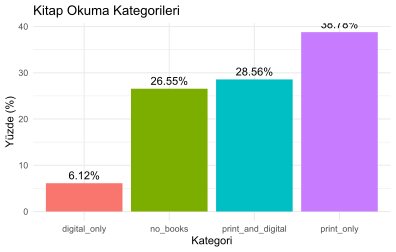
\includegraphics{4_hafta_tanimlayici_istatistik_files/figure-pdf/unnamed-chunk-3-1.pdf}

}

\end{figure}

\hypertarget{uxf6rnek-2-etnik-gruplar-ve-bilim-haberlerine-ilgi}{%
\subsubsection{\texorpdfstring{Örnek 2: \textbf{Etnik Gruplar ve Bilim
Haberlerine
İlgi}:}{Örnek 2: Etnik Gruplar ve Bilim Haberlerine İlgi:}}\label{uxf6rnek-2-etnik-gruplar-ve-bilim-haberlerine-ilgi}}

\begin{Shaded}
\begin{Highlighting}[]
\FunctionTok{library}\NormalTok{(dplyr)}
\FunctionTok{library}\NormalTok{(tidyr)}
\FunctionTok{library}\NormalTok{(ggplot2)}

\CommentTok{\# Veriler}
\NormalTok{white }\OtherTok{\textless{}{-}} \FunctionTok{c}\NormalTok{(}\StringTok{"active"}\OtherTok{=}\DecValTok{487}\NormalTok{, }\StringTok{"casual"}\OtherTok{=}\DecValTok{916}\NormalTok{, }\StringTok{"uninterested"}\OtherTok{=}\DecValTok{1431}\NormalTok{, }\StringTok{"no\_answer"}\OtherTok{=}\DecValTok{28}\NormalTok{)}
\NormalTok{black }\OtherTok{\textless{}{-}} \FunctionTok{c}\NormalTok{(}\StringTok{"active"}\OtherTok{=}\DecValTok{59}\NormalTok{, }\StringTok{"casual"}\OtherTok{=}\DecValTok{98}\NormalTok{, }\StringTok{"uninterested"}\OtherTok{=}\DecValTok{227}\NormalTok{, }\StringTok{"no\_answer"}\OtherTok{=}\DecValTok{8}\NormalTok{)}
\NormalTok{hispanic }\OtherTok{\textless{}{-}} \FunctionTok{c}\NormalTok{(}\StringTok{"active"}\OtherTok{=}\DecValTok{89}\NormalTok{, }\StringTok{"casual"}\OtherTok{=}\DecValTok{152}\NormalTok{, }\StringTok{"uninterested"}\OtherTok{=}\DecValTok{183}\NormalTok{, }\StringTok{"no\_answer"}\OtherTok{=}\DecValTok{23}\NormalTok{)}

\CommentTok{\# 1. Veri çerçevesi oluşturma}
\NormalTok{my\_table }\OtherTok{\textless{}{-}} \FunctionTok{as.data.frame}\NormalTok{(}\FunctionTok{rbind}\NormalTok{(white, black, hispanic))}

\CommentTok{\# 2. Oranları hesapla (satır bazında)}
\NormalTok{prop\_table }\OtherTok{\textless{}{-}} \FunctionTok{round}\NormalTok{(}\FunctionTok{prop.table}\NormalTok{(}\FunctionTok{as.matrix}\NormalTok{(my\_table), }\AttributeTok{margin =} \DecValTok{1}\NormalTok{) }\SpecialCharTok{*} \DecValTok{100}\NormalTok{, }\DecValTok{2}\NormalTok{)}
\NormalTok{prop\_table\_df }\OtherTok{\textless{}{-}} \FunctionTok{as.data.frame}\NormalTok{(prop\_table)}

\CommentTok{\# 3. Oranları tablo olarak görüntüle}
\NormalTok{prop\_table\_df}
\end{Highlighting}
\end{Shaded}

\begin{longtable}[]{@{}lrrrr@{}}
\toprule\noalign{}
& active & casual & uninterested & no\_answer \\
\midrule\noalign{}
\endhead
\bottomrule\noalign{}
\endlastfoot
white & 17.02 & 32.01 & 50.00 & 0.98 \\
black & 15.05 & 25.00 & 57.91 & 2.04 \\
hispanic & 19.91 & 34.00 & 40.94 & 5.15 \\
\end{longtable}

\begin{Shaded}
\begin{Highlighting}[]
\CommentTok{\# Uzun formata dönüştür}
\NormalTok{prop\_long }\OtherTok{\textless{}{-}}\NormalTok{ prop\_table\_df }\SpecialCharTok{\%\textgreater{}\%}
  \FunctionTok{rownames\_to\_column}\NormalTok{(}\AttributeTok{var =} \StringTok{"group"}\NormalTok{) }\SpecialCharTok{\%\textgreater{}\%}
  \FunctionTok{pivot\_longer}\NormalTok{(}\AttributeTok{cols =} \SpecialCharTok{{-}}\NormalTok{group, }\AttributeTok{names\_to =} \StringTok{"category"}\NormalTok{, }\AttributeTok{values\_to =} \StringTok{"percent"}\NormalTok{)}

\CommentTok{\# Bar Plot oluştur}
\FunctionTok{ggplot}\NormalTok{(prop\_long, }\FunctionTok{aes}\NormalTok{(}\AttributeTok{x =}\NormalTok{ group, }\AttributeTok{y =}\NormalTok{ percent, }\AttributeTok{fill =}\NormalTok{ category)) }\SpecialCharTok{+}
  \FunctionTok{geom\_col}\NormalTok{(}\AttributeTok{width =} \FloatTok{0.7}\NormalTok{) }\SpecialCharTok{+}
  \FunctionTok{geom\_text}\NormalTok{(}\FunctionTok{aes}\NormalTok{(}\AttributeTok{label =} \FunctionTok{paste0}\NormalTok{(percent, }\StringTok{"\%"}\NormalTok{)),}
            \AttributeTok{position =} \FunctionTok{position\_stack}\NormalTok{(}\AttributeTok{vjust =} \FloatTok{0.5}\NormalTok{),}
            \AttributeTok{size =} \FloatTok{3.5}\NormalTok{) }\SpecialCharTok{+}
  \FunctionTok{labs}\NormalTok{(}
    \AttributeTok{title =} \StringTok{"Etnik Gruplara Göre Bilim Haberlerine İlgi"}\NormalTok{,}
    \AttributeTok{x =} \StringTok{"Etnik Grup"}\NormalTok{,}
    \AttributeTok{y =} \StringTok{"Yüzde (\%)"}\NormalTok{,}
    \AttributeTok{fill =} \StringTok{"İlgi Kategorisi"}
\NormalTok{  ) }\SpecialCharTok{+}
  \FunctionTok{theme\_minimal}\NormalTok{(}\AttributeTok{base\_size =} \DecValTok{13}\NormalTok{)}
\end{Highlighting}
\end{Shaded}

\begin{figure}[H]

{\centering 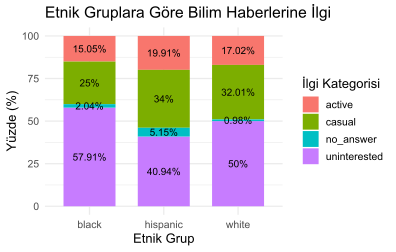
\includegraphics{4_hafta_tanimlayici_istatistik_files/figure-pdf/unnamed-chunk-5-1.pdf}

}

\end{figure}

\hypertarget{uxf6rnek-3-titanikte-hayatta-kalma-oranlarux131}{%
\subsubsection{Örnek 3: Titanik'te Hayatta Kalma
Oranları}\label{uxf6rnek-3-titanikte-hayatta-kalma-oranlarux131}}

\begin{Shaded}
\begin{Highlighting}[]
\CommentTok{\# Titanic verisini okuma}
\NormalTok{titanic }\OtherTok{\textless{}{-}} \FunctionTok{read.csv}\NormalTok{(}\StringTok{"https://raw.githubusercontent.com/bio304{-}class/bio304{-}course{-}notes/master/datasets/titanic\_data.csv"}\NormalTok{)}

\CommentTok{\# Gerekli kütüphaneleri yükleyin}
\FunctionTok{library}\NormalTok{(tidyverse)}

\CommentTok{\# Cinsiyet dağılımı tablosu}
\FunctionTok{table}\NormalTok{(titanic}\SpecialCharTok{$}\NormalTok{sex)}
\end{Highlighting}
\end{Shaded}

\begin{verbatim}

female   male 
   466    843 
\end{verbatim}

\begin{Shaded}
\begin{Highlighting}[]
\CommentTok{\# Cinsiyet dağılımını gösteren çubuk grafiği}
\FunctionTok{barplot}\NormalTok{(}\FunctionTok{table}\NormalTok{(titanic}\SpecialCharTok{$}\NormalTok{sex), }\AttributeTok{main =} \StringTok{"Cinsiyet Dağılımı"}\NormalTok{, }\AttributeTok{xlab =} \StringTok{"Cinsiyet"}\NormalTok{, }\AttributeTok{ylab =} \StringTok{"Frekans"}\NormalTok{, }\AttributeTok{col =} \StringTok{"lightblue"}\NormalTok{)}
\end{Highlighting}
\end{Shaded}

\begin{figure}[H]

{\centering \includegraphics{4_hafta_tanimlayici_istatistik_files/figure-pdf/unnamed-chunk-6-1.pdf}

}

\end{figure}

\begin{Shaded}
\begin{Highlighting}[]
\CommentTok{\# Hayatta kalma durumu tablosu}
\FunctionTok{table}\NormalTok{(titanic}\SpecialCharTok{$}\NormalTok{survived)}
\end{Highlighting}
\end{Shaded}

\begin{verbatim}

  0   1 
809 500 
\end{verbatim}

\begin{Shaded}
\begin{Highlighting}[]
\CommentTok{\# Hayatta kalma durumunu gösteren çubuk grafiği}
\FunctionTok{barplot}\NormalTok{(}\FunctionTok{table}\NormalTok{(titanic}\SpecialCharTok{$}\NormalTok{survived), }\AttributeTok{main =} \StringTok{"Hayatta Kalma Durumu"}\NormalTok{, }\AttributeTok{xlab =} \StringTok{"Hayatta Kalma"}\NormalTok{, }\AttributeTok{ylab =} \StringTok{"Frekans"}\NormalTok{, }\AttributeTok{col =} \StringTok{"lightgreen"}\NormalTok{)}
\end{Highlighting}
\end{Shaded}

\begin{figure}[H]

{\centering 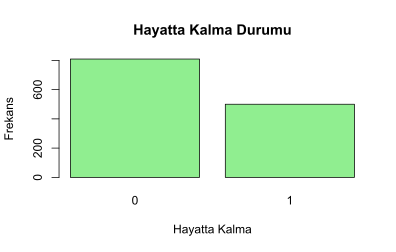
\includegraphics{4_hafta_tanimlayici_istatistik_files/figure-pdf/unnamed-chunk-6-2.pdf}

}

\end{figure}

\begin{Shaded}
\begin{Highlighting}[]
\CommentTok{\# Cinsiyet ve hayatta kalma durumu arasındaki tablo}
\NormalTok{table\_1 }\OtherTok{\textless{}{-}} \FunctionTok{table}\NormalTok{(titanic}\SpecialCharTok{$}\NormalTok{sex, titanic}\SpecialCharTok{$}\NormalTok{survived)}

\CommentTok{\# Toplamları ekleyerek tabloyu gösterme}
\FunctionTok{addmargins}\NormalTok{(table\_1)}
\end{Highlighting}
\end{Shaded}

\begin{verbatim}
        
            0    1  Sum
  female  127  339  466
  male    682  161  843
  Sum     809  500 1309
\end{verbatim}

\begin{Shaded}
\begin{Highlighting}[]
\CommentTok{\# Oran tablosunu gösterme}
\FunctionTok{prop.table}\NormalTok{(table\_1, }\AttributeTok{margin =} \DecValTok{2}\NormalTok{)}
\end{Highlighting}
\end{Shaded}

\begin{verbatim}
        
                 0         1
  female 0.1569839 0.6780000
  male   0.8430161 0.3220000
\end{verbatim}

\begin{Shaded}
\begin{Highlighting}[]
\CommentTok{\# Cinsiyet ve hayatta kalma durumu için çubuk grafiği}
\FunctionTok{barplot}\NormalTok{(table\_1, }\AttributeTok{legend.text =} \ConstantTok{TRUE}\NormalTok{, }\AttributeTok{main =} \StringTok{"Cinsiyet ve Hayatta Kalma"}\NormalTok{, }\AttributeTok{xlab =} \StringTok{"Cinsiyet"}\NormalTok{, }\AttributeTok{ylab =} \StringTok{"Frekans"}\NormalTok{)}
\end{Highlighting}
\end{Shaded}

\begin{figure}[H]

{\centering \includegraphics{4_hafta_tanimlayici_istatistik_files/figure-pdf/unnamed-chunk-6-3.pdf}

}

\end{figure}

\begin{Shaded}
\begin{Highlighting}[]
\CommentTok{\# Sınıf ve hayatta kalma durumu arasındaki tablo}
\NormalTok{table\_2 }\OtherTok{\textless{}{-}} \FunctionTok{table}\NormalTok{(titanic}\SpecialCharTok{$}\NormalTok{pclass, titanic}\SpecialCharTok{$}\NormalTok{survived)}

\CommentTok{\# Toplamları ekleyerek tabloyu gösterme}
\FunctionTok{addmargins}\NormalTok{(table\_2)}
\end{Highlighting}
\end{Shaded}

\begin{verbatim}
     
         0    1  Sum
  1    123  200  323
  2    158  119  277
  3    528  181  709
  Sum  809  500 1309
\end{verbatim}

\begin{Shaded}
\begin{Highlighting}[]
\CommentTok{\# Oran tablosunu gösterme}
\FunctionTok{prop.table}\NormalTok{(table\_2)}
\end{Highlighting}
\end{Shaded}

\begin{verbatim}
   
             0          1
  1 0.09396486 0.15278839
  2 0.12070283 0.09090909
  3 0.40336134 0.13827349
\end{verbatim}

\begin{Shaded}
\begin{Highlighting}[]
\CommentTok{\# Sınıf ve hayatta kalma durumu için çubuk grafiği}
\FunctionTok{barplot}\NormalTok{(table\_2, }\AttributeTok{legend.text =} \ConstantTok{TRUE}\NormalTok{, }\AttributeTok{main =} \StringTok{"Sınıf ve Hayatta Kalma"}\NormalTok{, }\AttributeTok{xlab =} \StringTok{"Sınıf"}\NormalTok{, }\AttributeTok{ylab =} \StringTok{"Frekans"}\NormalTok{)}
\end{Highlighting}
\end{Shaded}

\begin{figure}[H]

{\centering 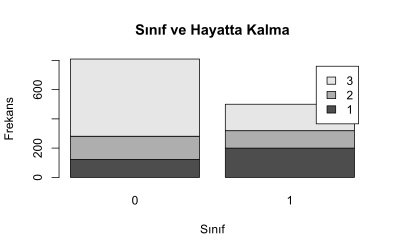
\includegraphics{4_hafta_tanimlayici_istatistik_files/figure-pdf/unnamed-chunk-6-4.pdf}

}

\end{figure}

\begin{Shaded}
\begin{Highlighting}[]
\CommentTok{\# Yaş ve hayatta kalma durumu arasındaki tablo}
\NormalTok{table\_3 }\OtherTok{\textless{}{-}} \FunctionTok{table}\NormalTok{(titanic}\SpecialCharTok{$}\NormalTok{age, titanic}\SpecialCharTok{$}\NormalTok{survived)}

\CommentTok{\# Toplamları ekleyerek tabloyu gösterme}
\FunctionTok{addmargins}\NormalTok{(table\_3)}
\end{Highlighting}
\end{Shaded}

\begin{verbatim}
        
            0    1  Sum
  0.1667    0    1    1
  0.3333    1    0    1
  0.4167    0    1    1
  0.6667    0    1    1
  0.75      1    2    3
  0.8333    0    3    3
  0.9167    0    2    2
  1         3    7   10
  2         8    4   12
  3         2    5    7
  4         3    7   10
  5         1    4    5
  6         3    3    6
  7         2    2    4
  8         2    4    6
  9         6    4   10
  10        4    0    4
  11        3    1    4
  11.5      1    0    1
  12        0    3    3
  13        2    3    5
  14        4    4    8
  14.5      2    0    2
  15        1    5    6
  16       11    8   19
  17       13    7   20
  18       25   14   39
  18.5      3    0    3
  19       18   11   29
  20       15    8   23
  20.5      1    0    1
  21       30   11   41
  22       23   20   43
  22.5      1    0    1
  23       16   10   26
  23.5      1    0    1
  24       25   22   47
  24.5      1    0    1
  25       23   11   34
  26       19   11   30
  26.5      1    0    1
  27       17   13   30
  28       24    8   32
  28.5      3    0    3
  29       17   13   30
  30       25   15   40
  30.5      2    0    2
  31       11   12   23
  32       13   11   24
  32.5      3    1    4
  33       12    9   21
  34       10    6   16
  34.5      2    0    2
  35       10   13   23
  36       17   14   31
  36.5      1    1    2
  37        7    2    9
  38        8    6   14
  38.5      1    0    1
  39       12    8   20
  40       12    6   18
  40.5      3    0    3
  41        9    2   11
  42       12    6   18
  43        6    3    9
  44        7    3   10
  45        7   14   21
  45.5      2    0    2
  46        6    0    6
  47       11    3   14
  48        4   10   14
  49        4    5    9
  50        9    6   15
  51        5    3    8
  52        3    3    6
  53        0    4    4
  54        5    5   10
  55        4    4    8
  55.5      1    0    1
  56        2    2    4
  57        5    0    5
  58        2    4    6
  59        2    1    3
  60        3    4    7
  60.5      1    0    1
  61        5    0    5
  62        3    2    5
  63        2    2    4
  64        3    2    5
  65        3    0    3
  66        1    0    1
  67        1    0    1
  70        2    0    2
  70.5      1    0    1
  71        2    0    2
  74        1    0    1
  76        0    1    1
  80        0    1    1
  Sum     619  427 1046
\end{verbatim}

\begin{Shaded}
\begin{Highlighting}[]
\CommentTok{\# Yaş dağılımını gösteren kutu grafiği}
\FunctionTok{boxplot}\NormalTok{(titanic}\SpecialCharTok{$}\NormalTok{age }\SpecialCharTok{\textasciitilde{}}\NormalTok{ titanic}\SpecialCharTok{$}\NormalTok{survived, }\AttributeTok{main =} \StringTok{"Yaş Dağılımı"}\NormalTok{, }\AttributeTok{xlab =} \StringTok{"Hayatta Kalma"}\NormalTok{, }\AttributeTok{ylab =} \StringTok{"Yaş"}\NormalTok{)}
\end{Highlighting}
\end{Shaded}

\begin{figure}[H]

{\centering \includegraphics{4_hafta_tanimlayici_istatistik_files/figure-pdf/unnamed-chunk-6-5.pdf}

}

\end{figure}

\textbf{Yorumlar:}

\begin{itemize}
\item
  \textbf{Grup 1}: 123 kişi ölmüş, 200 kişi hayatta kalmış. Toplamda 323
  kişi.
\item
  \textbf{Grup 2}: 158 kişi ölmüş, 119 kişi hayatta kalmış. Toplamda 277
  kişi.
\item
  \textbf{Grup 3}: 528 kişi ölmüş, 181 kişi hayatta kalmış. Toplamda 709
  kişi.
\item
  \textbf{Toplamlar}:

  \begin{itemize}
  \item
    Tüm gruplarda toplam 1309 kişi gözlemlenmiştir.
  \item
    Ölenlerin toplamı 809, hayatta kalanların toplamı ise 500'dür.
  \end{itemize}
\item
  \textbf{Hayatta Kalma Oranı}:

  \begin{itemize}
  \tightlist
  \item
    En yüksek hayatta kalma sayısına sahip grup 1'dir (200 kişi
    hayatta), en yüksek ölüm sayısına sahip grup ise 3'tür (528 kişi
    ölmüş).
  \end{itemize}
\item
  \textbf{Hayatta Kalma Oranları}: Kadınların hayatta kalma oranı
  (67.8\%) erkeklerin hayatta kalma oranından (32.2\%) oldukça
  yüksektir. Bu, kadınların Titanic faciasında erkeklere göre daha
  yüksek bir hayatta kalma oranına sahip olduğunu göstermektedir.
\item
  \textbf{Ölüm Oranları}: Erkekler için ölüm oranı (84.3\%) oldukça
  yüksekken, kadınlar için bu oran çok daha düşüktür (15.7\%). Bu durum,
  kadınların daha iyi korunmuş olabileceğini veya bazı sosyal
  faktörlerin etkisiyle hayatta kalma şanslarının artmış olabileceğini
  düşündürmektedir.
\end{itemize}

\hypertarget{sayux131sal-deux11fiux15fkenlerle-kullanux131labilen-tanux131mlayux131cux131-istatistikler}{%
\subsection{Sayısal Değişkenlerle Kullanılabilen Tanımlayıcı
İstatistikler}\label{sayux131sal-deux11fiux15fkenlerle-kullanux131labilen-tanux131mlayux131cux131-istatistikler}}

Tanımlayıcı istatistiklerde veriyi tanımlamak için sıkça kullanılan
istatistiksel ölçümler şunlardır:

\begin{enumerate}
\def\labelenumi{\arabic{enumi}.}
\item
  \textbf{Merkezi Eğilim Ölçüleri}: Ortalama, Medyan, Mod
\item
  \textbf{Merkezi Dağılım Ölçüleri}: Aralık, standart sapma, varyans
\item
  \textbf{Eğrilik ve Basıklık}: Dağılım grafiklerinin normal dağılımdan
  farklılaşması
\item
  \textbf{Korelasyon}: İki değişken arasındaki ilişkinin yönü ve gücü.
\end{enumerate}

\hypertarget{merkezi-eux11filim-uxf6luxe7uxfcleri}{%
\subsubsection{1. Merkezi Eğilim
Ölçüleri:}\label{merkezi-eux11filim-uxf6luxe7uxfcleri}}

\textbf{1.1 Ortalama (Mean)}:

\begin{itemize}
\item
  \textbf{Tanım}: Verilerin aritmetik ortalaması, tüm değerlerin
  toplamının gözlem sayısına bölünmesi ile hesaplanır.
\item
  \textbf{Matematiksel Gösterim}:
  \[\text{Ortalama} = \frac{\sum_{i=1}^{n} x_i}{n}\]
  \hspace{0pt}\hspace{0pt}
\item
  \textbf{R Formülü}:

\begin{Shaded}
\begin{Highlighting}[]
\NormalTok{veri }\OtherTok{\textless{}{-}} \FunctionTok{c}\NormalTok{(}\DecValTok{34}\NormalTok{, }\DecValTok{67}\NormalTok{, }\DecValTok{23}\NormalTok{, }\DecValTok{45}\NormalTok{, }\DecValTok{89}\NormalTok{, }\DecValTok{12}\NormalTok{, }\DecValTok{56}\NormalTok{, }\DecValTok{78}\NormalTok{, }\DecValTok{99}\NormalTok{, }\DecValTok{5}\NormalTok{, }\DecValTok{62}\NormalTok{, }\DecValTok{48}\NormalTok{, }\DecValTok{39}\NormalTok{, }\DecValTok{75}\NormalTok{, }\DecValTok{80}\NormalTok{, }\DecValTok{22}\NormalTok{, }\DecValTok{90}\NormalTok{, }\DecValTok{11}\NormalTok{, }\DecValTok{36}\NormalTok{, }\DecValTok{50}\NormalTok{)}

\FunctionTok{mean}\NormalTok{(veri)  }\CommentTok{\# veri, ortalamasını almak istediğiniz sayısal vektördür.}
\end{Highlighting}
\end{Shaded}

\begin{verbatim}
[1] 51.05
\end{verbatim}
\end{itemize}

\textbf{1.2 Medyan (Median)}:

\begin{itemize}
\tightlist
\item
  \textbf{Tanım}: Verilerin sıralandıktan sonra ortadaki değeri.
  Özellikle aşırı değerlerin etkisini azaltır.
\item
  \textbf{Matematiksel Gösterim}:

  \begin{itemize}
  \item
    \textbf{Eğer} n tek ise:

    \[
    \text{Medyan} = x_{\left(\frac{n+1}{2}\right)}
    \]
  \item
    \textbf{Eğer} n çift ise:

    \[
    \text{Medyan} = \frac{x_{\left(\frac{n}{2}\right)} + x_{\left(\frac{n}{2}+1\right)}}{2}
    \]
  \end{itemize}
\end{itemize}

\begin{Shaded}
\begin{Highlighting}[]
\FunctionTok{median}\NormalTok{(veri)  }\CommentTok{\# veri, medyanını almak istediğiniz sayısal vektördür.}
\end{Highlighting}
\end{Shaded}

\begin{verbatim}
[1] 49
\end{verbatim}

\begin{tcolorbox}[enhanced jigsaw, bottomrule=.15mm, opacitybacktitle=0.6, rightrule=.15mm, left=2mm, toprule=.15mm, leftrule=.75mm, titlerule=0mm, colframe=quarto-callout-note-color-frame, opacityback=0, arc=.35mm, colbacktitle=quarto-callout-note-color!10!white, title=\textcolor{quarto-callout-note-color}{\faInfo}\hspace{0.5em}{Not}, coltitle=black, breakable, bottomtitle=1mm, toptitle=1mm, colback=white]

⚠️ Ortalama, veri setinin ``ağırlık merkezi''dir: verilerin histogramını
katı bir cisim olarak hayal ederseniz, onu dengeleyebileceğiniz nokta
(bir tahterevalli gibi) ortalamadır. Buna karşılık, medyan ortadaki
gözlemdir. Gözlemlerin yarısı daha küçüktür ve yarısı daha büyüktür.

\end{tcolorbox}

\begin{figure}

{\centering \includegraphics{images/meanvsmedian.png}

}

\end{figure}

\textbf{1.3 Mod (Mode)}:

\begin{itemize}
\item
  \textbf{Tanım}: En sık rastlanan sayısal değer. Sayısal veriler için
  de kullanılabilir, ancak genellikle kategorik verilerle daha
  yaygındır.
\item
  \textbf{R Formülü:}
\end{itemize}

\begin{Shaded}
\begin{Highlighting}[]
\NormalTok{mode\_function }\OtherTok{\textless{}{-}} \ControlFlowTok{function}\NormalTok{(x) \{}
\NormalTok{  uniq\_x }\OtherTok{\textless{}{-}} \FunctionTok{unique}\NormalTok{(x)}
\NormalTok{  uniq\_x[}\FunctionTok{which.max}\NormalTok{(}\FunctionTok{tabulate}\NormalTok{(}\FunctionTok{match}\NormalTok{(x, uniq\_x)))]}
\NormalTok{\}}
\FunctionTok{mode\_function}\NormalTok{(veri)  }\CommentTok{\# veri, modunu almak istediğiniz sayısal vektördür.}
\end{Highlighting}
\end{Shaded}

\begin{verbatim}
[1] 34
\end{verbatim}

\hypertarget{merkezi-daux11fux131lux131m-uxf6luxe7uxfcleri}{%
\subsubsection{2. Merkezi Dağılım
Ölçüleri}\label{merkezi-daux11fux131lux131m-uxf6luxe7uxfcleri}}

\textbf{2.1 Aralık (Range)}:

\begin{itemize}
\item
  \textbf{Matematiksel Gösterim}: \[\text{Aralık} = \max(x) - \min(x)\]
\item
  \textbf{R Formülü:}
\end{itemize}

\begin{Shaded}
\begin{Highlighting}[]
\FunctionTok{range}\NormalTok{(veri)  }\CommentTok{\# veri, aralığını almak istediğiniz sayısal vektördür.}
\end{Highlighting}
\end{Shaded}

\begin{verbatim}
[1]  5 99
\end{verbatim}

\begin{Shaded}
\begin{Highlighting}[]
\FunctionTok{max}\NormalTok{(veri) }\SpecialCharTok{{-}} \FunctionTok{min}\NormalTok{(veri)  }\CommentTok{\# Aralığın hesaplanması}
\end{Highlighting}
\end{Shaded}

\begin{verbatim}
[1] 94
\end{verbatim}

\textbf{2.2 Standart Sapma (Standard Deviation)}:

\begin{itemize}
\item
  \textbf{Tanım:} Verilerin ortalamadan ne kadar yayıldığını gösterir.
  Verilerin ne kadar değişken olduğunu ölçer.
\item
  \textbf{Matematiksel Gösterim:}
  \[\text{Standart Sapma} = \sqrt{\frac{\sum_{i=1}^{n} (x_i - \bar{x})^2}{n-1}} \]
\item
  \textbf{R Formülü}
\end{itemize}

\begin{Shaded}
\begin{Highlighting}[]
\FunctionTok{sd}\NormalTok{(veri)  }\CommentTok{\# veri, standart sapmasını almak istediğiniz sayısal vektördür.}
\end{Highlighting}
\end{Shaded}

\begin{verbatim}
[1] 28.45398
\end{verbatim}

\textbf{2.3 Varyans (Variance)}:

\begin{itemize}
\item
  \textbf{Tanım}: Verilerin ortalamadan ne kadar saptığını gösteren bir
  ölçüdür. Standart sapmanın karesidir. Veriler arasındaki dağılımın ne
  kadar farklı olduğunu anlamamıza yardımcı olur. \textbf{Matematiksel
  Gösterim}:
  \[ \text{Varyans} = \frac{\sum_{i=1}^{n} (x_i - \bar{x})^2}{n-1}​\]
\item
  \textbf{R Formülü}
\end{itemize}

\begin{Shaded}
\begin{Highlighting}[]
\FunctionTok{var}\NormalTok{(veri)  }\CommentTok{\# veri, varyansını almak istediğiniz sayısal vektördür.}
\end{Highlighting}
\end{Shaded}

\begin{verbatim}
[1] 809.6289
\end{verbatim}

\begin{figure}

{\centering \includegraphics{images/varsdcal.png}

}

\end{figure}

\begin{figure}

{\centering \includegraphics{images/varsdtab.png}

}

\end{figure}

\textbf{2.4 Çeyrekler Aralığı (Interquartile Range, IQR)}:

\begin{itemize}
\item
  \textbf{Tanım}: Verilerin ortasındaki yarısını kapsayan yayılımı
  gösterir. 1. çeyrek (Q1) ile 3. çeyrek (Q3) arasındaki farktır.
\item
  \textbf{Matematiksel Gösterim}: \[ \text{IQR} = Q3 - Q1 \]
\item
  \textbf{R Formülü}
\end{itemize}

\begin{Shaded}
\begin{Highlighting}[]
\FunctionTok{IQR}\NormalTok{(veri)  }\CommentTok{\# veri, çeyrekler aralığını almak istediğiniz sayısal vektördür.}
\end{Highlighting}
\end{Shaded}

\begin{verbatim}
[1] 44.5
\end{verbatim}

\textbf{2.5 Küçük ve Büyük Çeyrekler (Quantiles)}:

\begin{itemize}
\item
  \textbf{Tanım:} Verilerin belirli bir yüzdesine karşılık gelen
  değerlerdir. Örneğin, \%25'lik çeyrek (Q1) ve \%75'lik çeyrek (Q3).
\item
  \textbf{R Formulü:}
\end{itemize}

\begin{Shaded}
\begin{Highlighting}[]
\FunctionTok{quantile}\NormalTok{(veri, }\AttributeTok{probs =} \FunctionTok{c}\NormalTok{(}\FloatTok{0.25}\NormalTok{, }\FloatTok{0.75}\NormalTok{))  }\CommentTok{\# \%25 ve \%75\textquotesingle{}lik çeyrekler}
\end{Highlighting}
\end{Shaded}

\begin{verbatim}
  25%   75% 
31.25 75.75 
\end{verbatim}

\hypertarget{daux11fux131lux131mda-sapma-eux11frilik-ve-basux131klux131k}{%
\subsubsection{\texorpdfstring{3. Dağılımda Sapma: \textbf{Eğrilik ve
Basıklık}}{3. Dağılımda Sapma: Eğrilik ve Basıklık}}\label{daux11fux131lux131mda-sapma-eux11frilik-ve-basux131klux131k}}

\textbf{3.1 Skewness (Eğrilik)}:

\begin{itemize}
\tightlist
\item
  \textbf{Tanım:} Verinin dağılımının simetrik olup olmadığını gösterir.
  Pozitif veya negatif eğrilik değerleri, veri dağılımının sağa veya
  sola kaydığını belirtir.
\end{itemize}

\includegraphics{images/skew.png}

\begin{tcolorbox}[enhanced jigsaw, bottomrule=.15mm, opacitybacktitle=0.6, rightrule=.15mm, left=2mm, toprule=.15mm, leftrule=.75mm, titlerule=0mm, colframe=quarto-callout-note-color-frame, opacityback=0, arc=.35mm, colbacktitle=quarto-callout-note-color!10!white, title=\textcolor{quarto-callout-note-color}{\faInfo}\hspace{0.5em}{Not}, coltitle=black, breakable, bottomtitle=1mm, toptitle=1mm, colback=white]

💡 Hertür eğrilikte Median daha merkezi bir tanımlayıcı istatistiğe
dönüşür.

\begin{figure}[H]

{\centering \includegraphics[width=6.94792in,height=\textheight]{images/relationship_between_mean_and_median_under_different_skewness8100144901166854637.png}

}

\end{figure}

\end{tcolorbox}

\textbf{3.2 Kurtosis (Basıklık)}:

\begin{itemize}
\tightlist
\item
  \textbf{Tanım:} Verinin dağılımının ne kadar ``keskin'' veya ``düz''
  olduğunu ölçer. Yüksek kurtosis, veri dağılımının keskin zirvelere
  sahip olduğunu gösterirken, düşük kurtosis daha düz bir dağılımı
  işaret eder.
\end{itemize}

\begin{figure}

{\centering \includegraphics{images/kurtosis.png}

}

\end{figure}

\begin{tcolorbox}[enhanced jigsaw, bottomrule=.15mm, opacitybacktitle=0.6, rightrule=.15mm, left=2mm, toprule=.15mm, leftrule=.75mm, titlerule=0mm, colframe=quarto-callout-note-color-frame, opacityback=0, arc=.35mm, colbacktitle=quarto-callout-note-color!10!white, title=\textcolor{quarto-callout-note-color}{\faInfo}\hspace{0.5em}{Not}, coltitle=black, breakable, bottomtitle=1mm, toptitle=1mm, colback=white]

Ortalama, Medyan, Mod, IQR ve Aralık (Range) Kullanım Rehberi

Veri analizi sırasında, ortalama, medyan, mod, çeyrekler aralığı (IQR)
ve aralık (range) gibi tanımlayıcı istatistikleri kullanarak
verilerimizi özetleyebiliriz. Ancak, her bir istatistiğin kullanımı,
veri setinin özelliklerine bağlıdır. Aşağıda, bu istatistiklerin hangi
durumlarda kullanılacağına dair detaylı bir rehber sunulmaktadır.

\begin{center}\rule{0.5\linewidth}{0.5pt}\end{center}

\textbf{1. Ortalama (Mean)}

\begin{itemize}
\item
  \textbf{Kullanım Durumu}: Sayısal verilerin merkezi eğilimini ölçmek
  için kullanılır.
\item
  \textbf{Uygun Durumlar}:

  \begin{itemize}
  \item
    Veriler normal dağılım gösteriyorsa.
  \item
    Aşırı değerler (outlier) yoksa.
  \end{itemize}
\item
  \textbf{Örnek}: Bir sınıfın notları 70, 75, 80, 85, 90 olduğunda
  ortalama 80'dir. Ancak, eğer sınıfta 0 alan bir öğrenci varsa (notlar:
  0, 70, 75, 80, 85, 90), ortalama 50 olur ki bu yanıltıcıdır.
\end{itemize}

\textbf{2. Medyan (Median)}

\begin{itemize}
\item
  \textbf{Kullanım Durumu}: Veri setinin ortasındaki değeri bulmak için
  kullanılır.
\item
  \textbf{Uygun Durumlar}:

  \begin{itemize}
  \item
    Veriler asimetrik dağılım gösteriyorsa.
  \item
    Aşırı değerler mevcutsa, çünkü medyan bu değerlerden etkilenmez.
  \end{itemize}
\item
  \textbf{Örnek}: Bir ev fiyatları seti 100.000, 120.000, 130.000,
  1.000.000, 1.200.000 olduğunda, ortalama fiyat 510.000, ancak medyan
  130.000'dir. Medyan, veri setinin çoğunluğunu daha iyi temsil eder.
\end{itemize}

\textbf{3. Mod (Mode)}

\begin{itemize}
\item
  \textbf{Kullanım Durumu}: En sık rastlanan değeri bulmak için
  kullanılır.
\item
  \textbf{Uygun Durumlar}:

  \begin{itemize}
  \item
    Kategorik verilerde kullanılır.
  \item
    Verilerin birden fazla mod değeri (bimodal veya multimodal) varsa.
  \end{itemize}
\item
  \textbf{Örnek}: Bir anket sonucu olarak, katılımcıların tercih ettiği
  meyveler: Elma, Muz, Elma, Portakal, Elma, Muz. Burada mod ``Elma''dır
  çünkü en sık rastlanan değerdir.
\end{itemize}

\textbf{4. Çeyrekler Aralığı (IQR)}

\begin{itemize}
\item
  \textbf{Kullanım Durumu}: Verilerin yayılımını ölçmek için kullanılır.
\item
  \textbf{Uygun Durumlar}:

  \begin{itemize}
  \item
    Verilerin ortasındaki yayılımı anlamak için.
  \item
    Aşırı değerlere karşı dayanıklıdır, bu yüzden özellikle asimetrik
    dağılımlarda tercih edilir.
  \end{itemize}
\item
  \textbf{Örnek}: Bir test notları setinde, 60, 70, 75, 80, 85, 90, 95,
  100 değerleri mevcutsa, IQR (Q3 - Q1) hesaplanarak veri setinin
  ortasında yer alan yayılım gösterilir. Q1 = 72.5 ve Q3 = 90 ise, IQR =
  90 - 72.5 = 17.5 olacaktır.
\end{itemize}

\textbf{5. Aralık (Range)}

\begin{itemize}
\item
  \textbf{Kullanım Durumu}: Verilerin en küçük ve en büyük değeri
  arasındaki farkı bulmak için kullanılır.
\item
  \textbf{Uygun Durumlar}:

  \begin{itemize}
  \item
    Veri setinin yayılımını genel olarak anlamak için.
  \item
    Aşırı değerlere dikkat edilmelidir, çünkü aralık bu değerlerden
    etkilenir.
  \end{itemize}
\item
  \textbf{Örnek}: Bir grup öğrencinin notları 50, 60, 70, 80, 90
  olduğunda, aralık 90 - 50 = 40'tır. Ancak, 0 alan bir öğrenci
  eklenirse (notlar: 0, 50, 60, 70, 80, 90), aralık 90 - 0 = 90
  olacaktır.
\end{itemize}

\begin{center}\rule{0.5\linewidth}{0.5pt}\end{center}

\textbf{Hangi İstatistiğin Kullanılacağına Dair Karar Verirken Dikkat
Edilmesi Gerekenler}

\begin{itemize}
\item
  \textbf{Veri Dağılımı}: Verilerin normal mi yoksa asimetrik mi
  dağıldığına bakın. Normal dağılımda ortalama kullanılabilirken,
  asimetrik dağılımda medyan daha iyi bir temsil sunar.
\item
  \textbf{Aşırı Değerler}: Veri setinde aşırı değerlerin (outlier) olup
  olmadığına dikkat edin. Aşırı değerlerin varlığında medyan ve IQR daha
  güvenilir ölçümler sağlar.
\item
  \textbf{Veri Türü}: Verilerin sayısal mı yoksa kategorik mi olduğunu
  belirleyin. Kategorik veriler için mod, sayısal veriler için ortalama
  ve medyan daha uygundur.
\item
  \textbf{Analiz Amacı}: Hangi bilgiyi elde etmek istediğinizi düşünün.
  Eğer yayılımı ölçmek istiyorsanız, IQR veya aralık kullanın; merkezi
  eğilimi ölçmek istiyorsanız, ortalama veya medyan tercih edin.
\end{itemize}

\end{tcolorbox}

\hypertarget{uxf6rnek-3-avustralya-futbol-ligi}{%
\subsubsection{Örnek 3: Avustralya Futbol
Ligi}\label{uxf6rnek-3-avustralya-futbol-ligi}}

\begin{Shaded}
\begin{Highlighting}[]
\FunctionTok{library}\NormalTok{(here)}
\FunctionTok{load}\NormalTok{(}\FunctionTok{here}\NormalTok{(}\StringTok{"data"}\NormalTok{, }\StringTok{"aflsmall.Rdata"}\NormalTok{))}

\CommentTok{\# Bu iki veri, Avustralya futbol ligi ile ilgilidir. afl.margins, 176 oyunun kazanç farkını içerir; afl.finalists ise 1987 ile 2010 arasında final oynayan 400 takımın isimlerini içerir. }

\FunctionTok{table}\NormalTok{(afl.finalists) }\CommentTok{\# Bu, bir vektördeki bir girişin kaç kez göründüğünü hesaplamak için tablo fonksiyonunu kullanır.}
\end{Highlighting}
\end{Shaded}

\begin{verbatim}
afl.finalists
        Adelaide         Brisbane          Carlton      Collingwood 
              26               25               26               28 
        Essendon          Fitzroy        Fremantle          Geelong 
              32                0                6               39 
        Hawthorn        Melbourne  North Melbourne    Port Adelaide 
              27               28               28               17 
        Richmond         St Kilda           Sydney       West Coast 
               6               24               26               38 
Western Bulldogs 
              24 
\end{verbatim}

\begin{Shaded}
\begin{Highlighting}[]
\FunctionTok{print}\NormalTok{(afl.margins)}
\end{Highlighting}
\end{Shaded}

\begin{verbatim}
  [1]  56  31  56   8  32  14  36  56  19   1   3 104  43  44  72   9  28  25
 [19]  27  55  20  16  16   7  23  40  48  64  22  55  95  15  49  52  50  10
 [37]  65  12  39  36   3  26  23  20  43 108  53  38   4   8   3  13  66  67
 [55]  50  61  36  38  29   9  81   3  26  12  36  37  70   1  35  12  50  35
 [73]   9  54  47   8  47   2  29  61  38  41  23  24   1   9  11  10  29  47
 [91]  71  38  49  65  18   0  16   9  19  36  60  24  25  44  55   3  57  83
[109]  84  35   4  35  26  22   2  14  19  30  19  68  11  75  48  32  36  39
[127]  50  11   0  63  82  26   3  82  73  19  33  48   8  10  53  20  71  75
[145]  76  54  44   5  22  94  29   8  98   9  89   1 101   7  21  52  42  21
[163] 116   3  44  29  27  16   6  44   3  28  38  29  10  10
\end{verbatim}

Verileri tanımlamak için bir histogram ile başlayalım. Bu, tanımlamaya
çalıştığımız verilerin nasıl göründüğüne dair bir fikir edinmenizi
sağlayacaktır.

\begin{Shaded}
\begin{Highlighting}[]
\CommentTok{\# Histogram oluşturma}
\FunctionTok{ggplot}\NormalTok{(}\AttributeTok{data =} \FunctionTok{data.frame}\NormalTok{(}\AttributeTok{margins =}\NormalTok{ afl.margins), }\FunctionTok{aes}\NormalTok{(}\AttributeTok{x =}\NormalTok{ margins)) }\SpecialCharTok{+}
  \FunctionTok{geom\_histogram}\NormalTok{(}\AttributeTok{bins =} \DecValTok{10}\NormalTok{, }\AttributeTok{fill =} \StringTok{"lightblue"}\NormalTok{, }\AttributeTok{color =} \StringTok{"black"}\NormalTok{, }\AttributeTok{alpha =} \FloatTok{0.7}\NormalTok{) }\SpecialCharTok{+}
  \FunctionTok{labs}\NormalTok{(}\AttributeTok{title =} \StringTok{"Kazanç Farklarının Histogramı"}\NormalTok{, }\AttributeTok{x =} \StringTok{"Kazanç Farkı"}\NormalTok{, }\AttributeTok{y =} \StringTok{"Frekans"}\NormalTok{) }\SpecialCharTok{+}
  \FunctionTok{theme\_minimal}\NormalTok{()}
\end{Highlighting}
\end{Shaded}

\begin{figure}[H]

{\centering \includegraphics{4_hafta_tanimlayici_istatistik_files/figure-pdf/unnamed-chunk-16-1.pdf}

}

\end{figure}

\begin{Shaded}
\begin{Highlighting}[]
\CommentTok{\# Tanımlayıcı istatistikleri hesaplama}
\NormalTok{ortalama }\OtherTok{\textless{}{-}} \FunctionTok{mean}\NormalTok{(afl.margins)}
\NormalTok{medyan }\OtherTok{\textless{}{-}} \FunctionTok{median}\NormalTok{(afl.margins)}

\CommentTok{\# Mod fonksiyonu tanımlama}
\NormalTok{mode\_function }\OtherTok{\textless{}{-}} \ControlFlowTok{function}\NormalTok{(x) \{}
\NormalTok{  uniq\_x }\OtherTok{\textless{}{-}} \FunctionTok{unique}\NormalTok{(x)}
\NormalTok{  uniq\_x[}\FunctionTok{which.max}\NormalTok{(}\FunctionTok{tabulate}\NormalTok{(}\FunctionTok{match}\NormalTok{(x, uniq\_x)))]}
\NormalTok{\}}
\NormalTok{mod }\OtherTok{\textless{}{-}} \FunctionTok{mode\_function}\NormalTok{(afl.margins)}

\NormalTok{varyans }\OtherTok{\textless{}{-}} \FunctionTok{var}\NormalTok{(afl.margins)}
\NormalTok{standart\_sapma }\OtherTok{\textless{}{-}} \FunctionTok{sd}\NormalTok{(afl.margins)}
\NormalTok{IQR\_val }\OtherTok{\textless{}{-}} \FunctionTok{IQR}\NormalTok{(afl.margins)}

\CommentTok{\# Sonuçları görüntüleme}
\NormalTok{result }\OtherTok{\textless{}{-}} \FunctionTok{data.frame}\NormalTok{(}
\NormalTok{  İ}\AttributeTok{statistik =} \FunctionTok{c}\NormalTok{(}\StringTok{"Ortalama"}\NormalTok{, }\StringTok{"Medyan"}\NormalTok{, }\StringTok{"Mod"}\NormalTok{, }\StringTok{"Varyans"}\NormalTok{, }\StringTok{"Standart Sapma"}\NormalTok{, }\StringTok{"Çeyrekler Aralığı"}\NormalTok{),}
\NormalTok{  Değer }\OtherTok{=} \FunctionTok{c}\NormalTok{(ortalama, medyan, mod, varyans, standart\_sapma, IQR\_val)}
\NormalTok{)}

\FunctionTok{print}\NormalTok{(result)}
\end{Highlighting}
\end{Shaded}

\begin{verbatim}
         İstatistik     Değer
1          Ortalama  35.30114
2            Medyan  30.50000
3               Mod   3.00000
4           Varyans 679.83451
5    Standart Sapma  26.07364
6 Çeyrekler Aralığı  37.75000
\end{verbatim}

\hypertarget{deux11fiux15fkenler-arasux131-iliux15fki-korelasyon}{%
\subsubsection{4. Değişkenler Arası İlişki:
Korelasyon}\label{deux11fiux15fkenler-arasux131-iliux15fki-korelasyon}}

Korelasyon, iki sayısal değişkenin doğrusal olarak ne derece ilişkili
olduğunu ifade eden istatistiksel bir ölçüttür (yani, iki değişkenin
birlikte sabit bir oranda değişip değişmediğini gösterir). Korelasyon,
basit ilişkileri tanımlamak için sıkça kullanılır ancak bu ilişki
hakkında bir nedensellik iddiasında bulunmaz; yalnızca iki değişkenin
nasıl birlikte hareket ettiğini gösterir.

Örneğin, sıcaklık arttıkça dondurma satışlarının da artması bir
korelasyon gösterebilir, ancak bu dondurma satışlarının artmasının
sebebinin sıcaklık olduğunu kesin olarak kanıtlamaz. Korelasyon,
genellikle -1 ile +1 arasında değişen bir korelasyon katsayısı (r) ile
ifade edilir.

\begin{itemize}
\item
  \textbf{Pozitif Korelasyon (r \textgreater{} 0):} Bir değişken
  arttıkça diğer değişken de artar. Örneğin, eğitim seviyesi ile gelir
  arasındaki ilişki genellikle pozitif korelasyon gösterir.
\item
  \textbf{Negatif Korelasyon (r \textless{} 0):} Bir değişken arttıkça
  diğer değişken azalır. Örneğin, bir araç ne kadar hız yaparsa
  gidebileceği mesafe o kadar azalır.
\item
  \textbf{Korelasyon Yok (r ≈ 0):} İki değişken arasında anlamlı bir
  doğrusal ilişki yoktur.
\end{itemize}

\hypertarget{uxf6rnek-4-ebeveyinlik}{%
\subsubsection{Örnek 4: Ebeveyinlik}\label{uxf6rnek-4-ebeveyinlik}}

Korelasyon hakkında daha ayrıntılı inceleme yapmak için yeni bir veri
seti kullanarak örneklemeye başlayalım:

\begin{Shaded}
\begin{Highlighting}[]
\CommentTok{\# veriyi yükle}
\FunctionTok{load}\NormalTok{(}\FunctionTok{here}\NormalTok{(}\StringTok{"data"}\NormalTok{, }\StringTok{"parenthood.Rdata"}\NormalTok{))}

\CommentTok{\# veriye göz at}
\FunctionTok{str}\NormalTok{(parenthood)}
\end{Highlighting}
\end{Shaded}

\begin{verbatim}
'data.frame':   100 obs. of  4 variables:
 $ dan.sleep : num  7.59 7.91 5.14 7.71 6.68 5.99 8.19 7.19 7.4 6.58 ...
 $ baby.sleep: num  10.18 11.66 7.92 9.61 9.75 ...
 $ dan.grump : num  56 60 82 55 67 72 53 60 60 71 ...
 $ day       : int  1 2 3 4 5 6 7 8 9 10 ...
\end{verbatim}

Öncelikle, \texttt{summary()} fonksiyonu ile veri setinin özetini
alabiliriz. Bu, her bir değişken için temel tanımlayıcı istatistikleri
(ortalama, medyan, minimum, maksimum, çeyrekler gibi) sağlar. Ardından,
bir değişkenin dağılımını görselleştirmek için \texttt{ggplot2}
kütüphanesini kullanarak histogram çizebiliriz.

\begin{Shaded}
\begin{Highlighting}[]
\CommentTok{\# Veri setinin özetini al}
\FunctionTok{summary}\NormalTok{(parenthood)}
\end{Highlighting}
\end{Shaded}

\begin{verbatim}
   dan.sleep       baby.sleep       dan.grump          day        
 Min.   :4.840   Min.   : 3.250   Min.   :41.00   Min.   :  1.00  
 1st Qu.:6.293   1st Qu.: 6.425   1st Qu.:57.00   1st Qu.: 25.75  
 Median :7.030   Median : 7.950   Median :62.00   Median : 50.50  
 Mean   :6.965   Mean   : 8.049   Mean   :63.71   Mean   : 50.50  
 3rd Qu.:7.740   3rd Qu.: 9.635   3rd Qu.:71.00   3rd Qu.: 75.25  
 Max.   :9.000   Max.   :12.070   Max.   :91.00   Max.   :100.00  
\end{verbatim}

\begin{Shaded}
\begin{Highlighting}[]
\CommentTok{\# Dan\textquotesingle{}in uyku süresi dağılımı histogramı}
\FunctionTok{ggplot}\NormalTok{(}\AttributeTok{data=}\NormalTok{parenthood, }\FunctionTok{aes}\NormalTok{(}\AttributeTok{x=}\NormalTok{dan.sleep)) }\SpecialCharTok{+} 
  \FunctionTok{geom\_histogram}\NormalTok{(}\AttributeTok{binwidth=}\DecValTok{1}\NormalTok{, }\AttributeTok{fill=}\StringTok{"blue"}\NormalTok{, }\AttributeTok{color=}\StringTok{"black"}\NormalTok{) }\SpecialCharTok{+}
  \FunctionTok{labs}\NormalTok{(}\AttributeTok{title=}\StringTok{"Dan\textquotesingle{}in Uyku Saatlerinin Dağılımı"}\NormalTok{, }\AttributeTok{x=}\StringTok{"Uyku Saatleri"}\NormalTok{, }\AttributeTok{y=}\StringTok{"Frekans"}\NormalTok{) }\SpecialCharTok{+}
  \FunctionTok{theme\_minimal}\NormalTok{()}
\end{Highlighting}
\end{Shaded}

\begin{figure}[H]

{\centering \includegraphics{4_hafta_tanimlayici_istatistik_files/figure-pdf/unnamed-chunk-20-1.pdf}

}

\end{figure}

\begin{Shaded}
\begin{Highlighting}[]
\CommentTok{\# Bebeğin uyku süresi dağılımı histogramı}
\FunctionTok{ggplot}\NormalTok{(}\AttributeTok{data=}\NormalTok{parenthood, }\FunctionTok{aes}\NormalTok{(}\AttributeTok{x=}\NormalTok{baby.sleep)) }\SpecialCharTok{+} 
  \FunctionTok{geom\_histogram}\NormalTok{(}\AttributeTok{binwidth=}\DecValTok{1}\NormalTok{, }\AttributeTok{fill=}\StringTok{"blue"}\NormalTok{, }\AttributeTok{color=}\StringTok{"black"}\NormalTok{) }\SpecialCharTok{+}
  \FunctionTok{labs}\NormalTok{(}\AttributeTok{title=}\StringTok{"Bebeğin Uyku Saatlerinin Dağılımı"}\NormalTok{, }\AttributeTok{x=}\StringTok{"Uyku Saatleri"}\NormalTok{, }\AttributeTok{y=}\StringTok{"Frekans"}\NormalTok{) }\SpecialCharTok{+}
  \FunctionTok{theme\_minimal}\NormalTok{()}
\end{Highlighting}
\end{Shaded}

\begin{figure}[H]

{\centering 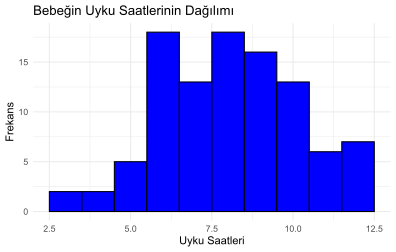
\includegraphics{4_hafta_tanimlayici_istatistik_files/figure-pdf/unnamed-chunk-21-1.pdf}

}

\end{figure}

\begin{Shaded}
\begin{Highlighting}[]
\CommentTok{\# Dan\textquotesingle{}in uyku süresi ile bebeğin uyku süresi arasındaki ilişki (korelasyon)}
\FunctionTok{ggplot}\NormalTok{(}\AttributeTok{data=}\NormalTok{parenthood, }\FunctionTok{aes}\NormalTok{(}\AttributeTok{x=}\NormalTok{dan.sleep, }\AttributeTok{y=}\NormalTok{baby.sleep)) }\SpecialCharTok{+}
  \FunctionTok{geom\_point}\NormalTok{() }\SpecialCharTok{+}
  \FunctionTok{labs}\NormalTok{(}\AttributeTok{title=}\StringTok{"Dan\textquotesingle{}in Uyku Süresi ile Bebeğin Uyku Süresi Arasındaki İlişki"}\NormalTok{, }\AttributeTok{x=}\StringTok{"Dan\textquotesingle{}in Uyku Süresi"}\NormalTok{, }\AttributeTok{y=}\StringTok{"Bebeğin Uyku Süresi"}\NormalTok{) }\SpecialCharTok{+}
  \FunctionTok{theme\_minimal}\NormalTok{()}
\end{Highlighting}
\end{Shaded}

\begin{figure}[H]

{\centering 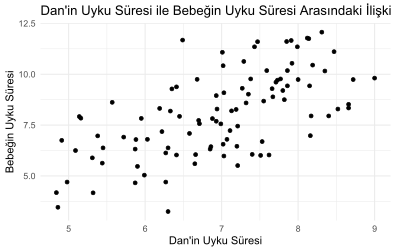
\includegraphics{4_hafta_tanimlayici_istatistik_files/figure-pdf/unnamed-chunk-22-1.pdf}

}

\end{figure}

\begin{Shaded}
\begin{Highlighting}[]
\CommentTok{\# Dan\textquotesingle{}in stres (grumpiness) seviyesinin dağılımı histogramı}
\FunctionTok{ggplot}\NormalTok{(}\AttributeTok{data=}\NormalTok{parenthood, }\FunctionTok{aes}\NormalTok{(}\AttributeTok{x=}\NormalTok{dan.grump)) }\SpecialCharTok{+}
  \FunctionTok{geom\_histogram}\NormalTok{(}\AttributeTok{binwidth=}\DecValTok{1}\NormalTok{, }\AttributeTok{fill=}\StringTok{"blue"}\NormalTok{, }\AttributeTok{color=}\StringTok{"black"}\NormalTok{) }\SpecialCharTok{+}
  \FunctionTok{labs}\NormalTok{(}\AttributeTok{title=}\StringTok{"Dan\textquotesingle{}in Stres Seviyesinin Dağılımı"}\NormalTok{, }\AttributeTok{x=}\StringTok{"Stres Seviyesi"}\NormalTok{, }\AttributeTok{y=}\StringTok{"Frekans"}\NormalTok{) }\SpecialCharTok{+}
  \FunctionTok{theme\_minimal}\NormalTok{()}
\end{Highlighting}
\end{Shaded}

\begin{figure}[H]

{\centering 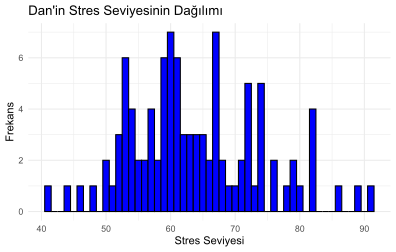
\includegraphics{4_hafta_tanimlayici_istatistik_files/figure-pdf/unnamed-chunk-23-1.pdf}

}

\end{figure}

\begin{Shaded}
\begin{Highlighting}[]
\CommentTok{\# Dan\textquotesingle{}in uyku süresi ile stres seviyesi arasındaki ilişki (korelasyon)}
\FunctionTok{ggplot}\NormalTok{(}\AttributeTok{data=}\NormalTok{parenthood, }\FunctionTok{aes}\NormalTok{(}\AttributeTok{x=}\NormalTok{dan.sleep, }\AttributeTok{y=}\NormalTok{dan.grump)) }\SpecialCharTok{+}
  \FunctionTok{geom\_point}\NormalTok{() }\SpecialCharTok{+}
  \FunctionTok{labs}\NormalTok{(}\AttributeTok{title=}\StringTok{"Dan\textquotesingle{}in Uyku Süresi ile Stres Seviyesi Arasındaki İlişki"}\NormalTok{, }\AttributeTok{x=}\StringTok{"Dan\textquotesingle{}in Uyku Süresi"}\NormalTok{, }\AttributeTok{y=}\StringTok{"Stres Seviyesi"}\NormalTok{) }\SpecialCharTok{+}
  \FunctionTok{theme\_minimal}\NormalTok{()}
\end{Highlighting}
\end{Shaded}

\begin{figure}[H]

{\centering 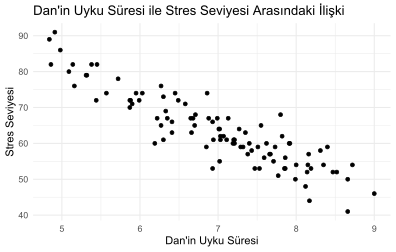
\includegraphics{4_hafta_tanimlayici_istatistik_files/figure-pdf/unnamed-chunk-24-1.pdf}

}

\end{figure}

\begin{Shaded}
\begin{Highlighting}[]
\CommentTok{\# parenthood veri setindeki tüm değişkenler arasındaki korelasyonları hesapla}
\NormalTok{korelasyon\_matrisi }\OtherTok{\textless{}{-}} \FunctionTok{cor}\NormalTok{(parenthood)}

\CommentTok{\# Korelasyon matrisini yazdır}
\FunctionTok{print}\NormalTok{(korelasyon\_matrisi)}
\end{Highlighting}
\end{Shaded}

\begin{verbatim}
             dan.sleep  baby.sleep   dan.grump         day
dan.sleep   1.00000000  0.62794934 -0.90338404 -0.09840768
baby.sleep  0.62794934  1.00000000 -0.56596373 -0.01043394
dan.grump  -0.90338404 -0.56596373  1.00000000  0.07647926
day        -0.09840768 -0.01043394  0.07647926  1.00000000
\end{verbatim}

\begin{tcolorbox}[enhanced jigsaw, bottomrule=.15mm, opacitybacktitle=0.6, rightrule=.15mm, left=2mm, toprule=.15mm, leftrule=.75mm, titlerule=0mm, colframe=quarto-callout-note-color-frame, opacityback=0, arc=.35mm, colbacktitle=quarto-callout-note-color!10!white, title=\textcolor{quarto-callout-note-color}{\faInfo}\hspace{0.5em}{Not}, coltitle=black, breakable, bottomtitle=1mm, toptitle=1mm, colback=white]

\textbf{Korelasyon Katsayısı:}

Korelasyon katsayısı, iki değişken arasındaki doğrusal ilişkinin yönünü
ve gücünü ölçen bir istatistiksel ölçüdür. -1 ile +1 arasında değerler
alır.

\begin{itemize}
\item
  \textbf{+1:} Mükemmel pozitif korelasyon. Bir değişken arttıkça, diğer
  değişken de aynı oranda artar. Görselde en alttaki sol grafikte
  görüldüğü gibi, tüm noktalar yükselen bir doğru üzerinde yer alır.
\item
  \textbf{+0.66:} Güçlü pozitif korelasyon. Bir değişken arttıkça, diğer
  değişken de genellikle artar, ancak mükemmel bir ilişki yoktur.
  Görselde ortadaki sol grafikte görüldüğü gibi, noktalar yükselen bir
  doğru etrafında kümelenmiştir, ancak doğrudan üzerinde değillerdir.
\item
  \textbf{+0.33:} Zayıf pozitif korelasyon. Bir değişken arttıkça, diğer
  değişkenin artma eğilimi vardır, ancak ilişki daha az belirgindir.
  Görselde üstteki sol grafikte görüldüğü gibi, noktalar dağınık bir
  şekilde yükselen bir trend gösterir.
\item
  \textbf{0:} Korelasyon yok. Değişkenler arasında doğrusal bir ilişki
  yoktur. Değişkenlerden birinin değeri değiştiğinde, diğerinin değeri
  üzerinde tahmin edilebilir bir etkisi olmaz.
\item
  \textbf{-0.33:} Zayıf negatif korelasyon. Bir değişken arttıkça, diğer
  değişkenin azalma eğilimi vardır. Görselde üstteki sağ grafikte
  görüldüğü gibi, noktalar dağınık bir şekilde azalan bir trend
  gösterir.
\item
  \textbf{-0.66:} Güçlü negatif korelasyon. Bir değişken arttıkça, diğer
  değişken genellikle azalır. Görselde ortadaki sağ grafikte görüldüğü
  gibi, noktalar azalan bir doğru etrafında kümelenmiştir.
\item
  \textbf{-1:} Mükemmel negatif korelasyon. Bir değişken arttıkça, diğer
  değişken aynı oranda azalır. Görselde en alttaki sağ grafikte
  görüldüğü gibi, tüm noktalar azalan bir doğru üzerinde yer alır.
\end{itemize}

\begin{figure}[H]

{\centering \includegraphics{images/correlation.png}

}

\end{figure}

\end{tcolorbox}

\hypertarget{korelasyon-bir-nedensellik-deux11fildir}{%
\paragraph{Korelasyon bir nedensellik
değildir}\label{korelasyon-bir-nedensellik-deux11fildir}}

Korelasyon, iki değişken arasındaki ilişkinin yönünü ve gücünü ifade
eder. Pozitif korelasyon, bir değişken arttığında diğerinin de artma
eğiliminde olduğunu, negatif korelasyon ise bir değişken arttığında
diğerinin azalma eğiliminde olduğunu gösterir.

\textbf{Önemli nokta:} Korelasyon, nedensellik anlamına gelmez. Yani,
iki değişken arasında korelasyon olması, birinin diğerine neden olduğu
anlamına gelmez.

\textbf{Örnek:} Dondurma satışları ile denizde boğulma vakaları arasında
pozitif bir korelasyon vardır. Yani, dondurma satışları arttığında,
boğulma vakaları da artar. Ancak bu, dondurma yemek insanların
boğulmasına neden oluyor anlamına gelmez. Aslında, her iki değişken de
sıcak hava gibi üçüncü bir faktörden etkilenir. Sıcak havalarda insanlar
daha çok dondurma yerler ve denize girerler, bu da boğulma vakalarının
artmasına neden olur.

\textbf{Başka bir örnek:} Ayakkabı numarası ile okuma becerileri
arasında pozitif bir korelasyon olabilir. Yani, ayakkabı numarası büyük
olan çocuklar genellikle daha iyi okuma becerilerine sahiptir. Ancak bu,
büyük ayakların çocukların daha iyi okumasına neden olduğu anlamına
gelmez. Aslında, her iki değişken de yaş gibi üçüncü bir faktörden
etkilenir. Çocuklar büyüdükçe ayakları büyür ve okuma becerileri
gelişir.

\textbf{Sonuç olarak:} Korelasyon, iki değişken arasında bir ilişki
olduğunu gösterir, ancak bu ilişkinin nedensel olup olmadığını
belirlemek için daha fazla araştırma yapmak gerekir.

\begin{Shaded}
\begin{Highlighting}[]
\CommentTok{\# "here" fonksiyonunu kullanabilmek için "here" paketini yükle}
\ControlFlowTok{if}\NormalTok{ (}\SpecialCharTok{!}\FunctionTok{require}\NormalTok{(}\StringTok{"here"}\NormalTok{)) }\FunctionTok{install.packages}\NormalTok{(}\StringTok{"here"}\NormalTok{)}

\CommentTok{\# Gerekli kütüphaneleri yükle}
\FunctionTok{library}\NormalTok{(here)}
\FunctionTok{library}\NormalTok{(ggplot2)}

\CommentTok{\# Veri setini yükle}
\FunctionTok{load}\NormalTok{(}\FunctionTok{here}\NormalTok{(}\StringTok{"data"}\NormalTok{, }\StringTok{"anscombesquartet.Rdata"}\NormalTok{))}

\CommentTok{\# X1, Y1, X2, Y2 vb. vektörlerini kullanarak bir data.frame oluştur}
\NormalTok{anscombesquartet }\OtherTok{\textless{}{-}} \FunctionTok{data.frame}\NormalTok{(X1, Y1, X2, Y2, X3, Y3, X4, Y4)}

\CommentTok{\# Farklı ikililer arası scatter plotlar oluştur}
\FunctionTok{ggplot}\NormalTok{(anscombesquartet, }\FunctionTok{aes}\NormalTok{(}\AttributeTok{x =}\NormalTok{ X1, }\AttributeTok{y =}\NormalTok{ Y1)) }\SpecialCharTok{+} 
  \FunctionTok{geom\_point}\NormalTok{() }\SpecialCharTok{+} 
  \FunctionTok{ggtitle}\NormalTok{(}\StringTok{"X1 ve Y1"}\NormalTok{)}
\end{Highlighting}
\end{Shaded}

\begin{figure}[H]

{\centering 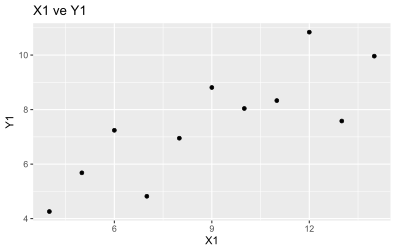
\includegraphics{4_hafta_tanimlayici_istatistik_files/figure-pdf/unnamed-chunk-26-1.pdf}

}

\end{figure}

\begin{Shaded}
\begin{Highlighting}[]
\FunctionTok{ggplot}\NormalTok{(anscombesquartet, }\FunctionTok{aes}\NormalTok{(}\AttributeTok{x =}\NormalTok{ X2, }\AttributeTok{y =}\NormalTok{ Y2)) }\SpecialCharTok{+} 
  \FunctionTok{geom\_point}\NormalTok{() }\SpecialCharTok{+} 
  \FunctionTok{ggtitle}\NormalTok{(}\StringTok{"X2 ve Y2"}\NormalTok{)}
\end{Highlighting}
\end{Shaded}

\begin{figure}[H]

{\centering 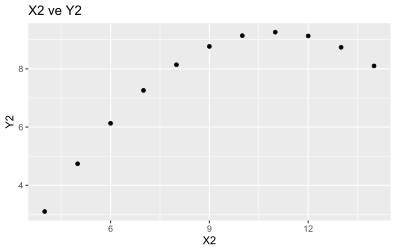
\includegraphics{4_hafta_tanimlayici_istatistik_files/figure-pdf/unnamed-chunk-26-2.pdf}

}

\end{figure}

\begin{Shaded}
\begin{Highlighting}[]
\FunctionTok{ggplot}\NormalTok{(anscombesquartet, }\FunctionTok{aes}\NormalTok{(}\AttributeTok{x =}\NormalTok{ X3, }\AttributeTok{y =}\NormalTok{ Y3)) }\SpecialCharTok{+} 
  \FunctionTok{geom\_point}\NormalTok{() }\SpecialCharTok{+} 
  \FunctionTok{ggtitle}\NormalTok{(}\StringTok{"X3 ve Y3"}\NormalTok{)}
\end{Highlighting}
\end{Shaded}

\begin{figure}[H]

{\centering 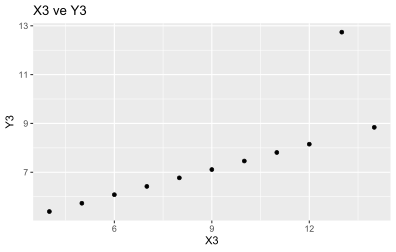
\includegraphics{4_hafta_tanimlayici_istatistik_files/figure-pdf/unnamed-chunk-26-3.pdf}

}

\end{figure}

\begin{Shaded}
\begin{Highlighting}[]
\FunctionTok{ggplot}\NormalTok{(anscombesquartet, }\FunctionTok{aes}\NormalTok{(}\AttributeTok{x =}\NormalTok{ X4, }\AttributeTok{y =}\NormalTok{ Y4)) }\SpecialCharTok{+} 
  \FunctionTok{geom\_point}\NormalTok{() }\SpecialCharTok{+} 
  \FunctionTok{ggtitle}\NormalTok{(}\StringTok{"X4 ve Y4"}\NormalTok{)}
\end{Highlighting}
\end{Shaded}

\begin{figure}[H]

{\centering 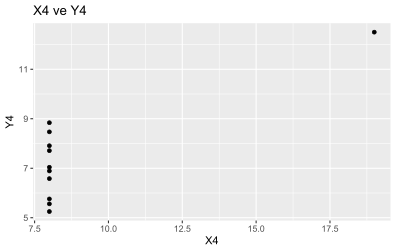
\includegraphics{4_hafta_tanimlayici_istatistik_files/figure-pdf/unnamed-chunk-26-4.pdf}

}

\end{figure}

\begin{Shaded}
\begin{Highlighting}[]
\CommentTok{\# Korelasyon katsayılarını hesapla}
\FunctionTok{cor}\NormalTok{(anscombesquartet}\SpecialCharTok{$}\NormalTok{X1, anscombesquartet}\SpecialCharTok{$}\NormalTok{Y1)}
\end{Highlighting}
\end{Shaded}

\begin{verbatim}
[1] 0.8164205
\end{verbatim}

\begin{Shaded}
\begin{Highlighting}[]
\FunctionTok{cor}\NormalTok{(anscombesquartet}\SpecialCharTok{$}\NormalTok{X2, anscombesquartet}\SpecialCharTok{$}\NormalTok{Y2)}
\end{Highlighting}
\end{Shaded}

\begin{verbatim}
[1] 0.8162365
\end{verbatim}

\begin{Shaded}
\begin{Highlighting}[]
\FunctionTok{cor}\NormalTok{(anscombesquartet}\SpecialCharTok{$}\NormalTok{X3, anscombesquartet}\SpecialCharTok{$}\NormalTok{Y3)}
\end{Highlighting}
\end{Shaded}

\begin{verbatim}
[1] 0.8162867
\end{verbatim}

\begin{Shaded}
\begin{Highlighting}[]
\FunctionTok{cor}\NormalTok{(anscombesquartet}\SpecialCharTok{$}\NormalTok{X4, anscombesquartet}\SpecialCharTok{$}\NormalTok{Y4)}
\end{Highlighting}
\end{Shaded}

\begin{verbatim}
[1] 0.8165214
\end{verbatim}

\begin{tcolorbox}[enhanced jigsaw, bottomrule=.15mm, opacitybacktitle=0.6, rightrule=.15mm, left=2mm, toprule=.15mm, leftrule=.75mm, titlerule=0mm, colframe=quarto-callout-note-color-frame, opacityback=0, arc=.35mm, colbacktitle=quarto-callout-note-color!10!white, title=\textcolor{quarto-callout-note-color}{\faInfo}\hspace{0.5em}{Not}, coltitle=black, breakable, bottomtitle=1mm, toptitle=1mm, colback=white]

👋 \textbf{Anscombe's Quartet veri seti neden önemli?}

Anscombe's Quartet, korelasyon katsayısının tek başına bir ilişkinin tam
resmini veremeyeceğini gösteren önemli bir örnektir. Dört veri kümesinin
de korelasyon katsayıları neredeyse aynıdır, ancak grafiklerine
baktığımızda çok farklı ilişkiler olduğunu görürüz:

\begin{itemize}
\item
  X1 ve Y1: Doğrusal bir ilişki var gibi görünüyor.
\item
  X2 ve Y2: Doğrusal bir ilişki yoktur, parabolik bir ilişki vardır.
\item
  X3 ve Y3: Doğrusal bir ilişki vardır, ancak bir aykırı değer bu
  ilişkiyi etkilemektedir.
\item
  X4 ve Y4: X4 neredeyse sabittir, tek bir aykırı değer Y4 ile yüksek
  bir korelasyon göstermektedir.
\end{itemize}

Bu nedenle, sadece korelasyon katsayısına bakmak yerine, verileri
görselleştirmek ve ilişkinin doğasını anlamak çok önemlidir.

\end{tcolorbox}

\begin{tcolorbox}[enhanced jigsaw, bottomrule=.15mm, opacitybacktitle=0.6, rightrule=.15mm, left=2mm, toprule=.15mm, leftrule=.75mm, titlerule=0mm, colframe=quarto-callout-note-color-frame, opacityback=0, arc=.35mm, colbacktitle=quarto-callout-note-color!10!white, title=\textcolor{quarto-callout-note-color}{\faInfo}\hspace{0.5em}{Not}, coltitle=black, breakable, bottomtitle=1mm, toptitle=1mm, colback=white]

💡 \textbf{\texttt{cor()} Fonksiyonunun \texttt{method} Parametresi}

R'daki \texttt{cor()} fonksiyonu, varsayılan olarak Pearson korelasyon
katsayısını hesaplar. Ancak, farklı korelasyon türleri hesaplamak
isteyebilirsiniz. İşte \texttt{method} parametresi ile
kullanabileceğiniz seçenekler:

\begin{itemize}
\tightlist
\item
  \textbf{``pearson''}: Pearson korelasyon katsayısı (varsayılan). İki
  değişken arasındaki doğrusal ilişkinin gücünü ölçer.
\item
  \textbf{``spearman''}: Spearman sıra korelasyon katsayısı.
  Değişkenlerin sıraları arasındaki korelasyonu ölçer. Doğrusal olmayan,
  monotonik ilişkilere duyarlıdır.
\item
  \textbf{``kendall''}: Kendall korelasyon katsayısı. İki değişken
  arasındaki uyum (concordance) sayısını temel alır. Aykırı değerlere
  karşı daha dayanıklıdır.
\end{itemize}

Örnek olarak, Spearman sıra korelasyonunu hesaplamak için \texttt{cor()}
fonksiyonunu şu şekilde kullanabilirsiniz:

\begin{Shaded}
\begin{Highlighting}[]
\FunctionTok{cor}\NormalTok{(x, y, }\AttributeTok{method =} \StringTok{"spearman"}\NormalTok{)}
\end{Highlighting}
\end{Shaded}

\textbf{Eksik Verilerle Başa Çıkma}

Veri setlerinde eksik veriler olması yaygın bir durumdur. \texttt{cor()}
fonksiyonu, eksik verilerle nasıl başa çıkacağını belirlemek için
\texttt{use} parametresini kullanır. İşte \texttt{use} parametresi ile
kullanabileceğiniz seçenekler:

\begin{itemize}
\tightlist
\item
  \textbf{``everything''}: Tüm gözlemleri kullanır. Eksik veri içeren
  herhangi bir çift, \texttt{NA} (Not Available) değeri üretir.
\item
  \textbf{``all.obs''}: Herhangi bir eksik veri varsa hata verir.
\item
  \textbf{``complete.obs''}: Eksik veri içeren gözlemleri tamamen
  çıkarır ve sadece tam gözlemleri kullanarak korelasyonu hesaplar.
\item
  \textbf{``na.or.complete''}: ``complete.obs'' ile aynıdır.
\item
  \textbf{``pairwise.complete.obs''}: Her bir değişken çifti için, eksik
  veri içeren gözlemleri çıkarır ve kalan gözlemlerle korelasyonu
  hesaplar.
\end{itemize}

Örnek olarak, eksik verileri olan gözlemleri çıkararak Pearson
korelasyonunu hesaplamak için \texttt{cor()} fonksiyonunu şu şekilde
kullanabilirsiniz:

\begin{Shaded}
\begin{Highlighting}[]
\FunctionTok{cor}\NormalTok{(x, y, }\AttributeTok{use =} \StringTok{"complete.obs"}\NormalTok{)}
\end{Highlighting}
\end{Shaded}

Eksik verilerle nasıl başa çıkılacağı, veri setinin özelliklerine ve
analiz amacına bağlıdır. Eksik verileri yok saymak veya yanlış
yöntemlerle doldurmak, yanıltıcı sonuçlara yol açabilir. Bu nedenle,
eksik verileri dikkatli bir şekilde ele almak önemlidir.

\end{tcolorbox}

\hypertarget{uxf6zet}{%
\subsection{Özet}\label{uxf6zet}}

Gerçek verileri analiz ederken yapacağınız ilk şeylerden biri temel
betimsel istatistikleri hesaplamaktır ve betimsel istatistikler,
çıkarımsal istatistiklerden çok daha kolay anlaşılır. Bu derste,
aşağıdaki konuları ele aldık:

\textbf{Merkezi eğilim ölçüleri:} Bu ölçüler, veri setinin tipik veya
merkezi bir değerini temsil etmeye çalışır. Ortalama, tüm değerlerin
toplamının değer sayısına bölünmesiyle elde edilir. Medyan, sıralanmış
veri setinin orta değeridir. Mod ise en sık görünen değerdir. Hangi
merkezi eğilim ölçüsünün kullanılacağı, verilerin dağılımına ve analiz
amacına bağlıdır.

\textbf{Merkezi dağılım ölçüleri:} Bu ölçüler, verilerin yayılımını veya
dağılımını gösterir. Aralık, en büyük değer ile en küçük değer
arasındaki farktır. Standart sapma, verilerin ortalamadan ne kadar
uzakta olduğunu gösterir. Çeyrekler arası aralık ise, veri setinin
\%25'i ile \%75'i arasındaki farktır.

\textbf{R'da değişkenlerin özetlerini alma:} Bu ders R'da veri analizi
yapmaya odaklandığından, R'da betimsel istatistiklerin nasıl
hesaplanacağı hakkında biraz zaman harcadık.

\textbf{Korelasyonlar:} İki sayısal değişken arasındaki ilişkinin yönünü
ve boyutunu incelemek üzere korelasyon hesaplamaları yaptık

\textbf{Eksik veriler:} Eksik veriler, veri analizinde yaygın bir
sorundur ve sonuçları etkileyebilir. Eksik verilerle başa çıkmak için
çeşitli yöntemler vardır, örneğin eksik verileri silmek, ortalama veya
medyan ile doldurmak veya daha gelişmiş istatistiksel yöntemler
kullanmak.



\end{document}
